\documentclass[twoside]{book}

% Packages required by doxygen
\usepackage{calc}
\usepackage{doxygen}
\usepackage{graphicx}
\usepackage[utf8]{inputenc}
\usepackage{makeidx}
\usepackage{multicol}
\usepackage{multirow}
\usepackage{textcomp}
\usepackage[table]{xcolor}

% Font selection
\usepackage[T1]{fontenc}
\usepackage{mathptmx}
\usepackage[scaled=.90]{helvet}
\usepackage{courier}
\usepackage{amssymb}
\usepackage{sectsty}
\renewcommand{\familydefault}{\sfdefault}
\allsectionsfont{%
  \fontseries{bc}\selectfont%
  \color{darkgray}%
}
\renewcommand{\DoxyLabelFont}{%
  \fontseries{bc}\selectfont%
  \color{darkgray}%
}

% Page & text layout
\usepackage{geometry}
\geometry{%
  a4paper,%
  top=2.5cm,%
  bottom=2.5cm,%
  left=2.5cm,%
  right=2.5cm%
}
\tolerance=750
\hfuzz=15pt
\hbadness=750
\setlength{\emergencystretch}{15pt}
\setlength{\parindent}{0cm}
\setlength{\parskip}{0.2cm}
\makeatletter
\renewcommand{\paragraph}{%
  \@startsection{paragraph}{4}{0ex}{-1.0ex}{1.0ex}{%
    \normalfont\normalsize\bfseries\SS@parafont%
  }%
}
\renewcommand{\subparagraph}{%
  \@startsection{subparagraph}{5}{0ex}{-1.0ex}{1.0ex}{%
    \normalfont\normalsize\bfseries\SS@subparafont%
  }%
}
\makeatother

% Headers & footers
\usepackage{fancyhdr}
\pagestyle{fancyplain}
\fancyhead[LE]{\fancyplain{}{\bfseries\thepage}}
\fancyhead[CE]{\fancyplain{}{}}
\fancyhead[RE]{\fancyplain{}{\bfseries\leftmark}}
\fancyhead[LO]{\fancyplain{}{\bfseries\rightmark}}
\fancyhead[CO]{\fancyplain{}{}}
\fancyhead[RO]{\fancyplain{}{\bfseries\thepage}}
\fancyfoot[LE]{\fancyplain{}{}}
\fancyfoot[CE]{\fancyplain{}{}}
\fancyfoot[RE]{\fancyplain{}{\bfseries\scriptsize Generated on Mon Nov 16 2015 20\-:42\-:30 for My Project by Doxygen }}
\fancyfoot[LO]{\fancyplain{}{\bfseries\scriptsize Generated on Mon Nov 16 2015 20\-:42\-:30 for My Project by Doxygen }}
\fancyfoot[CO]{\fancyplain{}{}}
\fancyfoot[RO]{\fancyplain{}{}}
\renewcommand{\footrulewidth}{0.4pt}
\renewcommand{\chaptermark}[1]{%
  \markboth{#1}{}%
}
\renewcommand{\sectionmark}[1]{%
  \markright{\thesection\ #1}%
}

% Indices & bibliography
\usepackage{natbib}
\usepackage[titles]{tocloft}
\setcounter{tocdepth}{3}
\setcounter{secnumdepth}{5}
\makeindex

% Hyperlinks (required, but should be loaded last)
\usepackage{ifpdf}
\ifpdf
  \usepackage[pdftex,pagebackref=true]{hyperref}
\else
  \usepackage[ps2pdf,pagebackref=true]{hyperref}
\fi
\hypersetup{%
  colorlinks=true,%
  linkcolor=blue,%
  citecolor=blue,%
  unicode%
}

% Custom commands
\newcommand{\clearemptydoublepage}{%
  \newpage{\pagestyle{empty}\cleardoublepage}%
}


%===== C O N T E N T S =====

\begin{document}

% Titlepage & ToC
\hypersetup{pageanchor=false}
\pagenumbering{roman}
\begin{titlepage}
\vspace*{7cm}
\begin{center}%
{\Large My Project }\\
\vspace*{1cm}
{\large Generated by Doxygen 1.8.6}\\
\vspace*{0.5cm}
{\small Mon Nov 16 2015 20:42:30}\\
\end{center}
\end{titlepage}
\clearemptydoublepage
\tableofcontents
\clearemptydoublepage
\pagenumbering{arabic}
\hypersetup{pageanchor=true}

%--- Begin generated contents ---
\chapter{Hierarchical Index}
\section{Class Hierarchy}
This inheritance list is sorted roughly, but not completely, alphabetically\-:\begin{DoxyCompactList}
\item \contentsline{section}{Base}{\pageref{classBase}}{}
\begin{DoxyCompactList}
\item \contentsline{section}{Photo}{\pageref{classPhoto}}{}
\item \contentsline{section}{Video}{\pageref{classVideo}}{}
\begin{DoxyCompactList}
\item \contentsline{section}{Film}{\pageref{classFilm}}{}
\end{DoxyCompactList}
\end{DoxyCompactList}
\item \contentsline{section}{T\-C\-P\-Server\-:\-:Callback}{\pageref{classTCPServer_1_1Callback}}{}
\begin{DoxyCompactList}
\item \contentsline{section}{T\-C\-P\-Server\-:\-:Callback\-Impl$<$ T $>$}{\pageref{classTCPServer_1_1CallbackImpl}}{}
\end{DoxyCompactList}
\item \contentsline{section}{Catalogue}{\pageref{classCatalogue}}{}
\item \contentsline{section}{Client}{\pageref{classClient}}{}
\item exception\begin{DoxyCompactList}
\item \contentsline{section}{Invalid\-Caracters}{\pageref{classInvalidCaracters}}{}
\end{DoxyCompactList}
\item \contentsline{section}{Input\-Buffer}{\pageref{structInputBuffer}}{}
\item list\begin{DoxyCompactList}
\item \contentsline{section}{Group}{\pageref{classGroup}}{}
\end{DoxyCompactList}
\item \contentsline{section}{T\-C\-P\-Server\-:\-:Lock}{\pageref{classTCPServer_1_1Lock}}{}
\item \contentsline{section}{My\-App}{\pageref{classMyApp}}{}
\item \contentsline{section}{Server\-Socket}{\pageref{classServerSocket}}{}
\item \contentsline{section}{Socket}{\pageref{classSocket}}{}
\item \contentsline{section}{Socket\-Buffer}{\pageref{classSocketBuffer}}{}
\begin{DoxyCompactList}
\item \contentsline{section}{T\-C\-P\-Server\-:\-:Cnx}{\pageref{classTCPServer_1_1Cnx}}{}
\end{DoxyCompactList}
\item \contentsline{section}{T\-C\-P\-Server}{\pageref{classTCPServer}}{}
\end{DoxyCompactList}

\chapter{Class Index}
\section{Class List}
Here are the classes, structs, unions and interfaces with brief descriptions\-:\begin{DoxyCompactList}
\item\contentsline{section}{\hyperlink{classBase}{Base} \\*The \hyperlink{classBase}{Base} class params\-: name\-: name of file including extension pathname\-: complete path to file methods\-: \hyperlink{classBase_accfd86f100d4232debfc745b2b244dbd}{set\-Name(string n)} \hyperlink{classBase_a257547bb1e92fe64fb01863d82c5db5d}{set\-Pathname(string p)} \hyperlink{classBase_a7608d0f3a0d939fdf1068883cd9f02cd}{get\-Name()} \hyperlink{classBase_a5987267cc60429ed6a65bd1e4ffa43ab}{get\-Pathname()} \hyperlink{classBase_a117954a5c2b7e6c040cbea5a98d81795}{open\-Object()} \hyperlink{classBase_ad712ff856464b0d3fa96d07eae70a90e}{affichage(ostream \&s)} }{\pageref{classBase}}{}
\item\contentsline{section}{\hyperlink{classTCPServer_1_1Callback}{T\-C\-P\-Server\-::\-Callback} }{\pageref{classTCPServer_1_1Callback}}{}
\item\contentsline{section}{\hyperlink{classTCPServer_1_1CallbackImpl}{T\-C\-P\-Server\-::\-Callback\-Impl$<$ T $>$} }{\pageref{classTCPServer_1_1CallbackImpl}}{}
\item\contentsline{section}{\hyperlink{classCatalogue}{Catalogue} \\*The \hyperlink{classCatalogue}{Catalogue} class Class containing a catalogue of multimedia and of groups. params\-: multimedia\-: map with a string as key and a \hyperlink{classBase}{Base} object groups\-: map with a string as key and a \hyperlink{classGroup}{Group} object methods\-: \hyperlink{classCatalogue_aba54aa202119c2184dc18e5278f3ae59}{create\-Photo(string n, string pathname, double lat, double lon)} \hyperlink{classCatalogue_a59e7c173b7b7b889bb531a9b1048119e}{create\-Video(string n, string pathname, int duree)} \hyperlink{classCatalogue_aeea731bce1425a52589a46f80af016c5}{create\-Film(string n, string pathname, int duree, unsigned int $\ast$tab, unsigned int num)} \hyperlink{classCatalogue_a9e834d56a00f43b03f598a5459966d00}{create\-Group(string n)} \hyperlink{classCatalogue_a88a9f6dcfac06d9a1eed7331ab3b1f40}{supprimer\-Multimedia(string p)} \hyperlink{classCatalogue_a1839ba57f687e559fcf0251a6841624b}{supprimer\-Group(string p)} \hyperlink{classCatalogue_a07fb093b33ce5fc95af3ea8874aeef97}{rechercher\-Multimedia(string p, ostream \&s)} \hyperlink{classCatalogue_ae033231c07cc7f5fd751a4c8d25ab8e5}{rechercher\-Group(string p, ostream \&s)} \hyperlink{classCatalogue_acb117d10f869d108f142cf38811f7022}{jouer(string p)} \hyperlink{classCatalogue_a47134c107bbda909706188dc759bc076}{save(const string \& file\-Name)} \hyperlink{classCatalogue_a9bba7adb9d7455f04b9cfc839c8ebd93}{load(const string \& file\-Name)} }{\pageref{classCatalogue}}{}
\item\contentsline{section}{\hyperlink{classClient}{Client} }{\pageref{classClient}}{}
\item\contentsline{section}{\hyperlink{classTCPServer_1_1Cnx}{T\-C\-P\-Server\-::\-Cnx} \\*Connection with a given client }{\pageref{classTCPServer_1_1Cnx}}{}
\item\contentsline{section}{\hyperlink{classFilm}{Film} \\*The \hyperlink{classFilm}{Film} class params\-: count\-: unsigned int $\ast$durees\-: unsigned int methods\-: \hyperlink{classFilm_acf9c4384117b17333e434d410914d48b}{set\-Durees(unsigned int $\ast$tab, unsigned int num)} \hyperlink{classFilm_a2beb91b3aa53d2b1f25e43783585aaf0}{get\-Durees()} \hyperlink{classFilm_a094ff01cf9629b9ec0bed4e6efd140d3}{get\-Nombre\-Chapitres()} \hyperlink{classFilm_a0fd2b4ba12627d9268fb0ee64b850b15}{affichage(ostream \& s)} }{\pageref{classFilm}}{}
\item\contentsline{section}{\hyperlink{classGroup}{Group} \\*The \hyperlink{classGroup}{Group} class params\-: name\-: string methods\-: \hyperlink{classGroup_a0c38a3d735a6bef446c1dceb27866408}{set\-Name(string n)} \hyperlink{classGroup_a030dc7b666d67a51926d6236c1707f14}{get\-Group\-Name()} \hyperlink{classGroup_ae5bd44de2616138eacca19189be39d3c}{affichage(ostream \& s)} }{\pageref{classGroup}}{}
\item\contentsline{section}{\hyperlink{structInputBuffer}{Input\-Buffer} }{\pageref{structInputBuffer}}{}
\item\contentsline{section}{\hyperlink{classInvalidCaracters}{Invalid\-Caracters} }{\pageref{classInvalidCaracters}}{}
\item\contentsline{section}{\hyperlink{classTCPServer_1_1Lock}{T\-C\-P\-Server\-::\-Lock} \\*Locks the server in read mode or in write mode. In order to avoid concurrency problems between threads, the callback method that processes requests should instantiate a \hyperlink{classTCPServer_1_1Lock}{Lock} object in the stack. The \hyperlink{classTCPServer_1_1Lock}{Lock} must be instantiated in write mode if the request changes data, or in read mode otherwise. A write lock blocks all other locks (hence, all other threads) until the callback method that issued the write lock returns }{\pageref{classTCPServer_1_1Lock}}{}
\item\contentsline{section}{\hyperlink{classMyApp}{My\-App} }{\pageref{classMyApp}}{}
\item\contentsline{section}{\hyperlink{classPhoto}{Photo} \\*The \hyperlink{classPhoto}{Photo} class params\-: lat\-: double lon\-: double methods\-: \hyperlink{classPhoto_a2a33bfd34dc606f17f4cb4ff1505afbe}{set\-Latitude(double la)} \hyperlink{classPhoto_a5846dcbc510174ed2db5cbbe99367a7f}{set\-Longitude(double lo)} \hyperlink{classPhoto_ac96f7a44787994f828e1fb24a4bdf768}{get\-Latitude()} \hyperlink{classPhoto_a736b26be1028d360f59800512b89b287}{get\-Longitude()} \hyperlink{classPhoto_a37b62ddde8114037efc2f8a8e97d0df0}{open\-Object()} \hyperlink{classPhoto_a2965c65d2ad33ebf2ac3b3cfad123fbb}{affichage(ostream \&s)} }{\pageref{classPhoto}}{}
\item\contentsline{section}{\hyperlink{classServerSocket}{Server\-Socket} \\*T\-C\-P/\-I\-P \hyperlink{classSocket}{Socket} Server. This class encapsulates a T\-C\-P/\-I\-P socket server. A\-F\-\_\-\-I\-N\-E\-T connections following the I\-Pv4 Internet protocol are supported }{\pageref{classServerSocket}}{}
\item\contentsline{section}{\hyperlink{classSocket}{Socket} \\*T\-C\-P/\-I\-P or U\-D\-P/\-Datagram \hyperlink{classSocket}{Socket}. This class encapsulates a T\-C\-P/\-I\-P or U\-D\-P/\-Datagram socket. A\-F\-\_\-\-I\-N\-E\-T connections following the I\-Pv4 Internet protocol are supported }{\pageref{classSocket}}{}
\item\contentsline{section}{\hyperlink{classSocketBuffer}{Socket\-Buffer} \\*Class for exchanging text strings between T\-C\-P/\-I\-P sockets. T\-C\-P/\-I\-P connected sockets do not preserve record boundaries. Messages can be split or merged so that one call to \hyperlink{classSocket_a9275eacdb64056a53cf4b9cf54cd2f1a}{Socket\-::send()} on the sending side does not necessarily correspond to one call to \hyperlink{classSocket_aa5e98b6f2c4e26fcf90d71c8386fc09d}{Socket\-::receive()} on the receiving side }{\pageref{classSocketBuffer}}{}
\item\contentsline{section}{\hyperlink{classTCPServer}{T\-C\-P\-Server} \\*T\-C\-P/\-I\-P I\-Pv4 server. The server supports T\-C\-P/\-I\-P A\-F\-\_\-\-I\-N\-E\-T connections (following the I\-Pv4 Internet protocol) with multiple clients. One thread is used per client }{\pageref{classTCPServer}}{}
\item\contentsline{section}{\hyperlink{classVideo}{Video} \\*The \hyperlink{classVideo}{Video} class params\-: duree\-: int methods\-: \hyperlink{classVideo_af9bf19109d8c613426173524942a59f0}{set\-Duree(int d)} \hyperlink{classVideo_a6ce28ec6b467212e7bb3cbf635b57598}{get\-Duree()} \hyperlink{classVideo_af6a8d2f22330651f3f264292e580dca3}{open\-Object()} \hyperlink{classVideo_a180c985ff368f77d0fb66ec106106f00}{affichage(ostream \&s)} }{\pageref{classVideo}}{}
\end{DoxyCompactList}

\chapter{Class Documentation}
\hypertarget{classBase}{\section{Base Class Reference}
\label{classBase}\index{Base@{Base}}
}


The \hyperlink{classBase}{Base} class params\-: name\-: name of file including extension pathname\-: complete path to file methods\-: \hyperlink{classBase_accfd86f100d4232debfc745b2b244dbd}{set\-Name(string n)} \hyperlink{classBase_a257547bb1e92fe64fb01863d82c5db5d}{set\-Pathname(string p)} \hyperlink{classBase_a7608d0f3a0d939fdf1068883cd9f02cd}{get\-Name()} \hyperlink{classBase_a5987267cc60429ed6a65bd1e4ffa43ab}{get\-Pathname()} \hyperlink{classBase_a117954a5c2b7e6c040cbea5a98d81795}{open\-Object()} \hyperlink{classBase_ad712ff856464b0d3fa96d07eae70a90e}{affichage(ostream \&s)}  




{\ttfamily \#include $<$base.\-h$>$}

Inheritance diagram for Base\-:\begin{figure}[H]
\begin{center}
\leavevmode
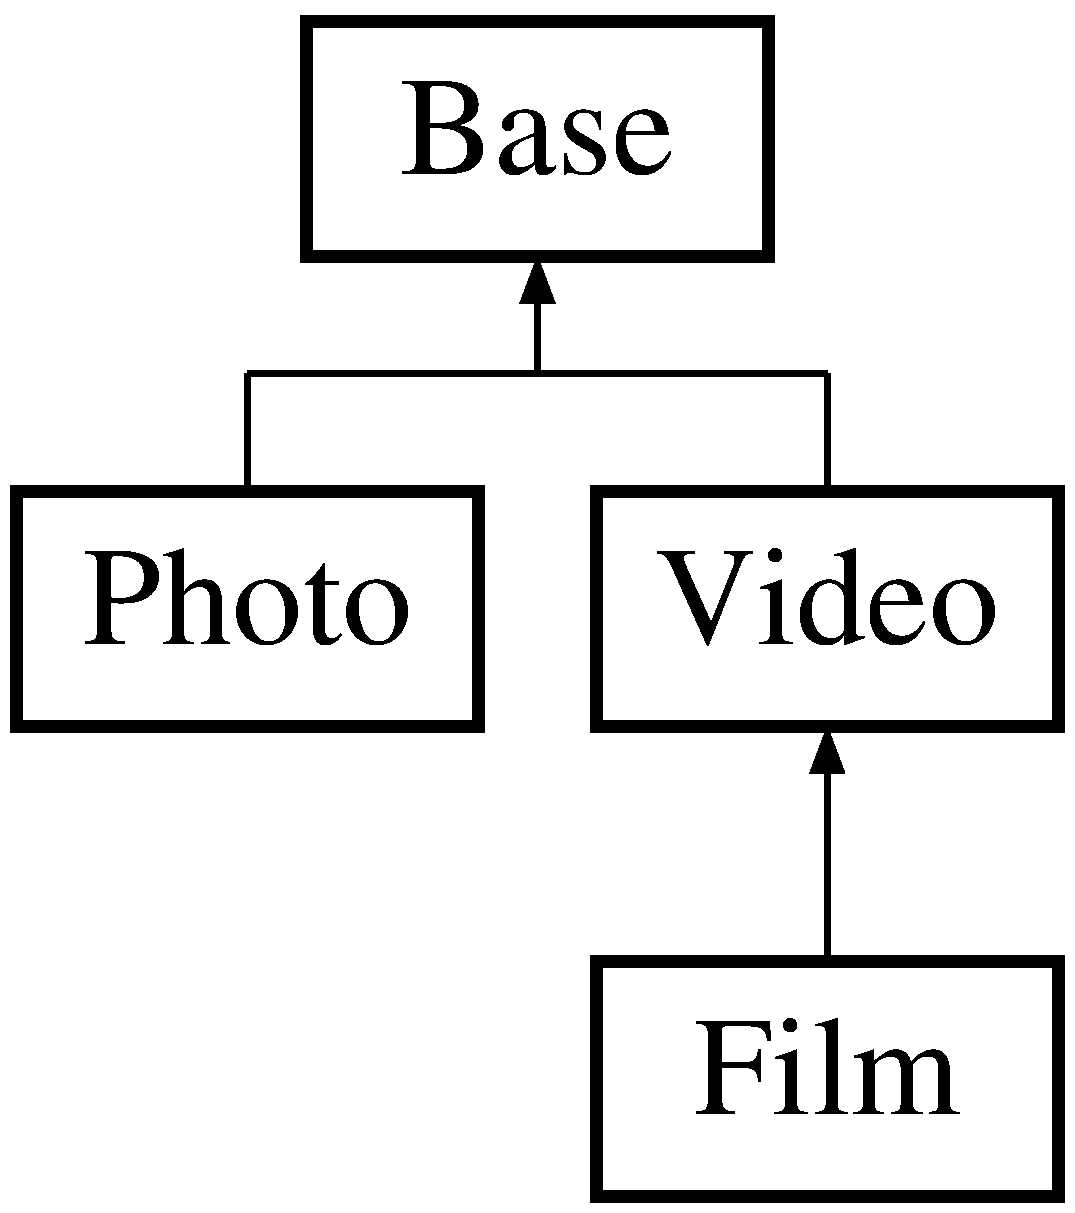
\includegraphics[height=3.000000cm]{classBase}
\end{center}
\end{figure}
\subsection*{Public Member Functions}
\begin{DoxyCompactItemize}
\item 
\hyperlink{classBase_aa44896f1e8d46be11fe7698a9a6947e0}{Base} (string name, string pathname)
\begin{DoxyCompactList}\small\item\em \hyperlink{classBase}{Base} constructor. \end{DoxyCompactList}\item 
\hypertarget{classBase_a5ffe0568374d8b9b4c4ec32953fd6453}{\hyperlink{classBase_a5ffe0568374d8b9b4c4ec32953fd6453}{Base} ()}\label{classBase_a5ffe0568374d8b9b4c4ec32953fd6453}

\begin{DoxyCompactList}\small\item\em \hyperlink{classBase}{Base} overcharge constructor. \end{DoxyCompactList}\item 
virtual void \hyperlink{classBase_accfd86f100d4232debfc745b2b244dbd}{set\-Name} (string n)
\begin{DoxyCompactList}\small\item\em set\-Name \end{DoxyCompactList}\item 
virtual void \hyperlink{classBase_a257547bb1e92fe64fb01863d82c5db5d}{set\-Pathname} (string p)
\begin{DoxyCompactList}\small\item\em set\-Pathname \end{DoxyCompactList}\item 
virtual string \hyperlink{classBase_a7608d0f3a0d939fdf1068883cd9f02cd}{get\-Name} () const 
\begin{DoxyCompactList}\small\item\em get\-Name \end{DoxyCompactList}\item 
virtual string \hyperlink{classBase_a5987267cc60429ed6a65bd1e4ffa43ab}{get\-Pathname} () const 
\begin{DoxyCompactList}\small\item\em get\-Pathname \end{DoxyCompactList}\item 
\hypertarget{classBase_a117954a5c2b7e6c040cbea5a98d81795}{virtual void \hyperlink{classBase_a117954a5c2b7e6c040cbea5a98d81795}{open\-Object} ()}\label{classBase_a117954a5c2b7e6c040cbea5a98d81795}

\begin{DoxyCompactList}\small\item\em open\-Object opens the object with the default program \end{DoxyCompactList}\item 
virtual string \hyperlink{classBase_ad712ff856464b0d3fa96d07eae70a90e}{affichage} (ostream \&s)
\begin{DoxyCompactList}\small\item\em affichage \end{DoxyCompactList}\item 
\hypertarget{classBase_a722da881b6c70cfcbde9243abcfbf334}{virtual \hyperlink{classBase_a722da881b6c70cfcbde9243abcfbf334}{$\sim$\-Base} ()}\label{classBase_a722da881b6c70cfcbde9243abcfbf334}

\begin{DoxyCompactList}\small\item\em $\sim$\-Base destructor \end{DoxyCompactList}\end{DoxyCompactItemize}


\subsection{Detailed Description}
The \hyperlink{classBase}{Base} class params\-: name\-: name of file including extension pathname\-: complete path to file methods\-: \hyperlink{classBase_accfd86f100d4232debfc745b2b244dbd}{set\-Name(string n)} \hyperlink{classBase_a257547bb1e92fe64fb01863d82c5db5d}{set\-Pathname(string p)} \hyperlink{classBase_a7608d0f3a0d939fdf1068883cd9f02cd}{get\-Name()} \hyperlink{classBase_a5987267cc60429ed6a65bd1e4ffa43ab}{get\-Pathname()} \hyperlink{classBase_a117954a5c2b7e6c040cbea5a98d81795}{open\-Object()} \hyperlink{classBase_ad712ff856464b0d3fa96d07eae70a90e}{affichage(ostream \&s)} 

\subsection{Constructor \& Destructor Documentation}
\hypertarget{classBase_aa44896f1e8d46be11fe7698a9a6947e0}{\index{Base@{Base}!Base@{Base}}
\index{Base@{Base}!Base@{Base}}
\subsubsection[{Base}]{\setlength{\rightskip}{0pt plus 5cm}Base\-::\-Base (
\begin{DoxyParamCaption}
\item[{string}]{name, }
\item[{string}]{pathname}
\end{DoxyParamCaption}
)}}\label{classBase_aa44896f1e8d46be11fe7698a9a6947e0}


\hyperlink{classBase}{Base} constructor. 


\begin{DoxyParams}{Parameters}
{\em name} & \\
\hline
{\em pathname} & \\
\hline
\end{DoxyParams}


\subsection{Member Function Documentation}
\hypertarget{classBase_ad712ff856464b0d3fa96d07eae70a90e}{\index{Base@{Base}!affichage@{affichage}}
\index{affichage@{affichage}!Base@{Base}}
\subsubsection[{affichage}]{\setlength{\rightskip}{0pt plus 5cm}string Base\-::affichage (
\begin{DoxyParamCaption}
\item[{ostream \&}]{s}
\end{DoxyParamCaption}
)\hspace{0.3cm}{\ttfamily [virtual]}}}\label{classBase_ad712ff856464b0d3fa96d07eae70a90e}


affichage 


\begin{DoxyParams}{Parameters}
{\em s} & ostream \\
\hline
\end{DoxyParams}
\begin{DoxyReturn}{Returns}
string with the attributes of the object Also prints through s the string 
\end{DoxyReturn}


Reimplemented in \hyperlink{classPhoto_a2965c65d2ad33ebf2ac3b3cfad123fbb}{Photo}, \hyperlink{classFilm_a0fd2b4ba12627d9268fb0ee64b850b15}{Film}, and \hyperlink{classVideo_a180c985ff368f77d0fb66ec106106f00}{Video}.

\hypertarget{classBase_a7608d0f3a0d939fdf1068883cd9f02cd}{\index{Base@{Base}!get\-Name@{get\-Name}}
\index{get\-Name@{get\-Name}!Base@{Base}}
\subsubsection[{get\-Name}]{\setlength{\rightskip}{0pt plus 5cm}string Base\-::get\-Name (
\begin{DoxyParamCaption}
{}
\end{DoxyParamCaption}
) const\hspace{0.3cm}{\ttfamily [virtual]}}}\label{classBase_a7608d0f3a0d939fdf1068883cd9f02cd}


get\-Name 

\begin{DoxyReturn}{Returns}
string with name of the file (including extension) 
\end{DoxyReturn}
\hypertarget{classBase_a5987267cc60429ed6a65bd1e4ffa43ab}{\index{Base@{Base}!get\-Pathname@{get\-Pathname}}
\index{get\-Pathname@{get\-Pathname}!Base@{Base}}
\subsubsection[{get\-Pathname}]{\setlength{\rightskip}{0pt plus 5cm}string Base\-::get\-Pathname (
\begin{DoxyParamCaption}
{}
\end{DoxyParamCaption}
) const\hspace{0.3cm}{\ttfamily [virtual]}}}\label{classBase_a5987267cc60429ed6a65bd1e4ffa43ab}


get\-Pathname 

\begin{DoxyReturn}{Returns}
string with path to the file 
\end{DoxyReturn}
\hypertarget{classBase_accfd86f100d4232debfc745b2b244dbd}{\index{Base@{Base}!set\-Name@{set\-Name}}
\index{set\-Name@{set\-Name}!Base@{Base}}
\subsubsection[{set\-Name}]{\setlength{\rightskip}{0pt plus 5cm}void Base\-::set\-Name (
\begin{DoxyParamCaption}
\item[{string}]{n}
\end{DoxyParamCaption}
)\hspace{0.3cm}{\ttfamily [virtual]}}}\label{classBase_accfd86f100d4232debfc745b2b244dbd}


set\-Name 


\begin{DoxyParams}{Parameters}
{\em n} & string Sets the name of the file (with extension) to the string n \\
\hline
\end{DoxyParams}
\hypertarget{classBase_a257547bb1e92fe64fb01863d82c5db5d}{\index{Base@{Base}!set\-Pathname@{set\-Pathname}}
\index{set\-Pathname@{set\-Pathname}!Base@{Base}}
\subsubsection[{set\-Pathname}]{\setlength{\rightskip}{0pt plus 5cm}void Base\-::set\-Pathname (
\begin{DoxyParamCaption}
\item[{string}]{p}
\end{DoxyParamCaption}
)\hspace{0.3cm}{\ttfamily [virtual]}}}\label{classBase_a257547bb1e92fe64fb01863d82c5db5d}


set\-Pathname 


\begin{DoxyParams}{Parameters}
{\em p} & string Sets the pathname of the file to the string p \\
\hline
\end{DoxyParams}


The documentation for this class was generated from the following files\-:\begin{DoxyCompactItemize}
\item 
base.\-h\item 
base.\-cpp\end{DoxyCompactItemize}

\hypertarget{classTCPServer_1_1Callback}{\section{T\-C\-P\-Server\-:\-:Callback Class Reference}
\label{classTCPServer_1_1Callback}\index{T\-C\-P\-Server\-::\-Callback@{T\-C\-P\-Server\-::\-Callback}}
}
Inheritance diagram for T\-C\-P\-Server\-:\-:Callback\-:\begin{figure}[H]
\begin{center}
\leavevmode
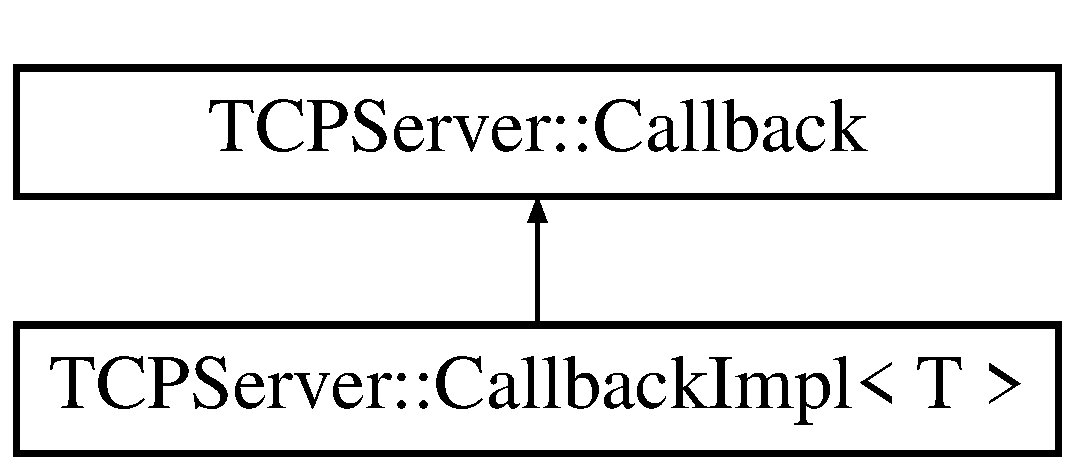
\includegraphics[height=2.000000cm]{classTCPServer_1_1Callback}
\end{center}
\end{figure}
\subsection*{Public Member Functions}
\begin{DoxyCompactItemize}
\item 
\hypertarget{classTCPServer_1_1Callback_a0d26469a5cfb3f5f0b3529cacb5d1615}{virtual bool {\bfseries call\-Func} (\hyperlink{classTCPServer_1_1Cnx}{Cnx} \&cnx, const std\-::string \&request, std\-::string \&response)=0}\label{classTCPServer_1_1Callback_a0d26469a5cfb3f5f0b3529cacb5d1615}

\end{DoxyCompactItemize}


The documentation for this class was generated from the following file\-:\begin{DoxyCompactItemize}
\item 
T\-C\-P\-Server.\-h\end{DoxyCompactItemize}

\hypertarget{classTCPServer_1_1CallbackImpl}{\section{T\-C\-P\-Server\-:\-:Callback\-Impl$<$ T $>$ Class Template Reference}
\label{classTCPServer_1_1CallbackImpl}\index{T\-C\-P\-Server\-::\-Callback\-Impl$<$ T $>$@{T\-C\-P\-Server\-::\-Callback\-Impl$<$ T $>$}}
}
Inheritance diagram for T\-C\-P\-Server\-:\-:Callback\-Impl$<$ T $>$\-:\begin{figure}[H]
\begin{center}
\leavevmode
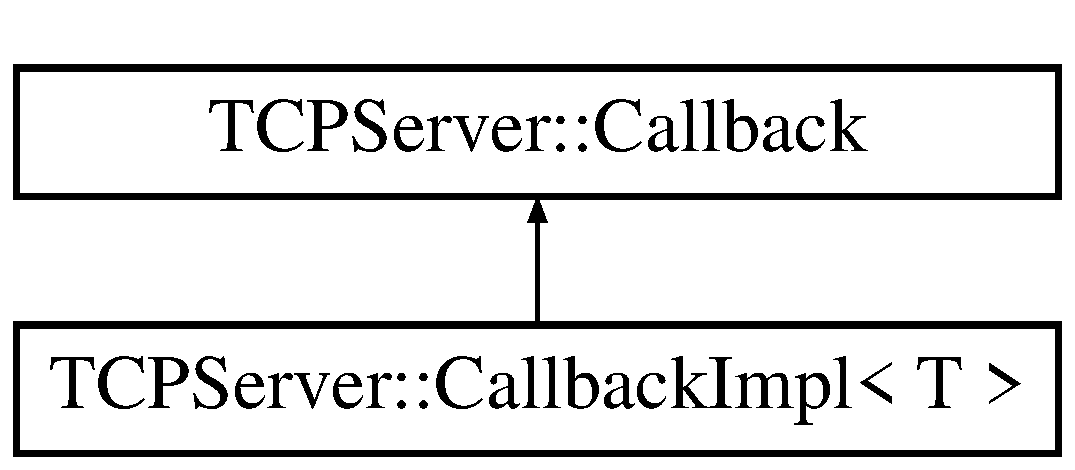
\includegraphics[height=2.000000cm]{classTCPServer_1_1CallbackImpl}
\end{center}
\end{figure}
\subsection*{Public Member Functions}
\begin{DoxyCompactItemize}
\item 
\hypertarget{classTCPServer_1_1CallbackImpl_a39abe4ac0e2782d2ec0504a01fcdeb1e}{{\bfseries Callback\-Impl} (T $\ast$obj, Func func)}\label{classTCPServer_1_1CallbackImpl_a39abe4ac0e2782d2ec0504a01fcdeb1e}

\item 
\hypertarget{classTCPServer_1_1CallbackImpl_a7370ad2f2dc50df8f623480f1991381b}{virtual bool {\bfseries call\-Func} (\hyperlink{classTCPServer_1_1Cnx}{Cnx} \&cnx, const std\-::string \&request, std\-::string \&response)}\label{classTCPServer_1_1CallbackImpl_a7370ad2f2dc50df8f623480f1991381b}

\end{DoxyCompactItemize}


The documentation for this class was generated from the following file\-:\begin{DoxyCompactItemize}
\item 
T\-C\-P\-Server.\-h\end{DoxyCompactItemize}

\hypertarget{classCatalogue}{\section{Catalogue Class Reference}
\label{classCatalogue}\index{Catalogue@{Catalogue}}
}


The \hyperlink{classCatalogue}{Catalogue} class Class containing a catalogue of multimedia and of groups. params\-: multimedia\-: map with a string as key and a \hyperlink{classBase}{Base} object groups\-: map with a string as key and a \hyperlink{classGroup}{Group} object methods\-: \hyperlink{classCatalogue_aba54aa202119c2184dc18e5278f3ae59}{create\-Photo(string n, string pathname, double lat, double lon)} \hyperlink{classCatalogue_a59e7c173b7b7b889bb531a9b1048119e}{create\-Video(string n, string pathname, int duree)} \hyperlink{classCatalogue_aeea731bce1425a52589a46f80af016c5}{create\-Film(string n, string pathname, int duree, unsigned int $\ast$tab, unsigned int num)} \hyperlink{classCatalogue_a9e834d56a00f43b03f598a5459966d00}{create\-Group(string n)} \hyperlink{classCatalogue_a88a9f6dcfac06d9a1eed7331ab3b1f40}{supprimer\-Multimedia(string p)} \hyperlink{classCatalogue_a1839ba57f687e559fcf0251a6841624b}{supprimer\-Group(string p)} \hyperlink{classCatalogue_a07fb093b33ce5fc95af3ea8874aeef97}{rechercher\-Multimedia(string p, ostream \&s)} \hyperlink{classCatalogue_ae033231c07cc7f5fd751a4c8d25ab8e5}{rechercher\-Group(string p, ostream \&s)} \hyperlink{classCatalogue_acb117d10f869d108f142cf38811f7022}{jouer(string p)} \hyperlink{classCatalogue_a47134c107bbda909706188dc759bc076}{save(const string \& file\-Name)} \hyperlink{classCatalogue_a9bba7adb9d7455f04b9cfc839c8ebd93}{load(const string \& file\-Name)}  




{\ttfamily \#include $<$catalogue.\-h$>$}

\subsection*{Public Member Functions}
\begin{DoxyCompactItemize}
\item 
\hyperlink{classCatalogue_a406ca1384645f90d84076fa8b3f4b3f2}{Catalogue} ()
\begin{DoxyCompactList}\small\item\em \hyperlink{classCatalogue}{Catalogue} Constructor. \end{DoxyCompactList}\item 
virtual void \hyperlink{classCatalogue_aba54aa202119c2184dc18e5278f3ae59}{create\-Photo} (string n, string pathname, double lat, double lon)
\begin{DoxyCompactList}\small\item\em create\-Photo \end{DoxyCompactList}\item 
virtual void \hyperlink{classCatalogue_a59e7c173b7b7b889bb531a9b1048119e}{create\-Video} (string n, string pathname, int duree)
\begin{DoxyCompactList}\small\item\em create\-Video \end{DoxyCompactList}\item 
virtual void \hyperlink{classCatalogue_aeea731bce1425a52589a46f80af016c5}{create\-Film} (string n, string pathname, int duree, unsigned int $\ast$tab, unsigned int num)
\begin{DoxyCompactList}\small\item\em create\-Film \end{DoxyCompactList}\item 
virtual void \hyperlink{classCatalogue_a9e834d56a00f43b03f598a5459966d00}{create\-Group} (string n)
\begin{DoxyCompactList}\small\item\em create\-Group \end{DoxyCompactList}\item 
virtual void \hyperlink{classCatalogue_a88a9f6dcfac06d9a1eed7331ab3b1f40}{supprimer\-Multimedia} (string p)
\begin{DoxyCompactList}\small\item\em supprimer\-Multimedia \end{DoxyCompactList}\item 
virtual void \hyperlink{classCatalogue_a1839ba57f687e559fcf0251a6841624b}{supprimer\-Group} (string p)
\begin{DoxyCompactList}\small\item\em supprimer\-Group \end{DoxyCompactList}\item 
virtual string \hyperlink{classCatalogue_a07fb093b33ce5fc95af3ea8874aeef97}{rechercher\-Multimedia} (string p, ostream \&s)
\begin{DoxyCompactList}\small\item\em rechercher\-Multimedia \end{DoxyCompactList}\item 
virtual string \hyperlink{classCatalogue_ae033231c07cc7f5fd751a4c8d25ab8e5}{rechercher\-Group} (string p, ostream \&s)
\begin{DoxyCompactList}\small\item\em rechercher\-Group \end{DoxyCompactList}\item 
virtual void \hyperlink{classCatalogue_acb117d10f869d108f142cf38811f7022}{jouer} (string p)
\begin{DoxyCompactList}\small\item\em jouer \end{DoxyCompactList}\item 
bool \hyperlink{classCatalogue_a47134c107bbda909706188dc759bc076}{save} (const string \&file\-Name)
\begin{DoxyCompactList}\small\item\em save \end{DoxyCompactList}\item 
bool \hyperlink{classCatalogue_a9bba7adb9d7455f04b9cfc839c8ebd93}{load} (const string \&file\-Name)
\begin{DoxyCompactList}\small\item\em load \end{DoxyCompactList}\item 
virtual \hyperlink{classCatalogue_a023fd8d70a58f76d2bbd6ef1e3ef0e9e}{$\sim$\-Catalogue} ()
\begin{DoxyCompactList}\small\item\em $\sim$\-Catalogue Destructor \end{DoxyCompactList}\end{DoxyCompactItemize}


\subsection{Detailed Description}
The \hyperlink{classCatalogue}{Catalogue} class Class containing a catalogue of multimedia and of groups. params\-: multimedia\-: map with a string as key and a \hyperlink{classBase}{Base} object groups\-: map with a string as key and a \hyperlink{classGroup}{Group} object methods\-: \hyperlink{classCatalogue_aba54aa202119c2184dc18e5278f3ae59}{create\-Photo(string n, string pathname, double lat, double lon)} \hyperlink{classCatalogue_a59e7c173b7b7b889bb531a9b1048119e}{create\-Video(string n, string pathname, int duree)} \hyperlink{classCatalogue_aeea731bce1425a52589a46f80af016c5}{create\-Film(string n, string pathname, int duree, unsigned int $\ast$tab, unsigned int num)} \hyperlink{classCatalogue_a9e834d56a00f43b03f598a5459966d00}{create\-Group(string n)} \hyperlink{classCatalogue_a88a9f6dcfac06d9a1eed7331ab3b1f40}{supprimer\-Multimedia(string p)} \hyperlink{classCatalogue_a1839ba57f687e559fcf0251a6841624b}{supprimer\-Group(string p)} \hyperlink{classCatalogue_a07fb093b33ce5fc95af3ea8874aeef97}{rechercher\-Multimedia(string p, ostream \&s)} \hyperlink{classCatalogue_ae033231c07cc7f5fd751a4c8d25ab8e5}{rechercher\-Group(string p, ostream \&s)} \hyperlink{classCatalogue_acb117d10f869d108f142cf38811f7022}{jouer(string p)} \hyperlink{classCatalogue_a47134c107bbda909706188dc759bc076}{save(const string \& file\-Name)} \hyperlink{classCatalogue_a9bba7adb9d7455f04b9cfc839c8ebd93}{load(const string \& file\-Name)} 

\subsection{Constructor \& Destructor Documentation}
\hypertarget{classCatalogue_a406ca1384645f90d84076fa8b3f4b3f2}{\index{Catalogue@{Catalogue}!Catalogue@{Catalogue}}
\index{Catalogue@{Catalogue}!Catalogue@{Catalogue}}
\subsubsection[{Catalogue}]{\setlength{\rightskip}{0pt plus 5cm}Catalogue\-::\-Catalogue (
\begin{DoxyParamCaption}
{}
\end{DoxyParamCaption}
)}}\label{classCatalogue_a406ca1384645f90d84076fa8b3f4b3f2}


\hyperlink{classCatalogue}{Catalogue} Constructor. 

\hyperlink{classCatalogue_a406ca1384645f90d84076fa8b3f4b3f2}{Catalogue\-::\-Catalogue}. \hypertarget{classCatalogue_a023fd8d70a58f76d2bbd6ef1e3ef0e9e}{\index{Catalogue@{Catalogue}!$\sim$\-Catalogue@{$\sim$\-Catalogue}}
\index{$\sim$\-Catalogue@{$\sim$\-Catalogue}!Catalogue@{Catalogue}}
\subsubsection[{$\sim$\-Catalogue}]{\setlength{\rightskip}{0pt plus 5cm}Catalogue\-::$\sim$\-Catalogue (
\begin{DoxyParamCaption}
{}
\end{DoxyParamCaption}
)\hspace{0.3cm}{\ttfamily [virtual]}}}\label{classCatalogue_a023fd8d70a58f76d2bbd6ef1e3ef0e9e}


$\sim$\-Catalogue Destructor 

\hyperlink{classCatalogue_a023fd8d70a58f76d2bbd6ef1e3ef0e9e}{Catalogue\-::$\sim$\-Catalogue}. 

\subsection{Member Function Documentation}
\hypertarget{classCatalogue_aeea731bce1425a52589a46f80af016c5}{\index{Catalogue@{Catalogue}!create\-Film@{create\-Film}}
\index{create\-Film@{create\-Film}!Catalogue@{Catalogue}}
\subsubsection[{create\-Film}]{\setlength{\rightskip}{0pt plus 5cm}void Catalogue\-::create\-Film (
\begin{DoxyParamCaption}
\item[{string}]{n, }
\item[{string}]{pathname, }
\item[{int}]{duree, }
\item[{unsigned int $\ast$}]{tab, }
\item[{unsigned int}]{num}
\end{DoxyParamCaption}
)\hspace{0.3cm}{\ttfamily [virtual]}}}\label{classCatalogue_aeea731bce1425a52589a46f80af016c5}


create\-Film 

\hyperlink{classCatalogue_aeea731bce1425a52589a46f80af016c5}{Catalogue\-::create\-Film}.


\begin{DoxyParams}{Parameters}
{\em n} & string \\
\hline
{\em pathname} & string \\
\hline
{\em duree} & int \\
\hline
{\em tab} & unsigned int \\
\hline
{\em num} & unsigned int Creates a film with the parameters given\\
\hline
{\em n} & \\
\hline
{\em pathname} & \\
\hline
{\em duree} & \\
\hline
{\em tab} & \\
\hline
{\em num} & Creates a new film with smart pointers Checks if there are other objects with the same name and shows error message Checks if the durees is zero or less and shows error message Checks for invalid characters \\
\hline
\end{DoxyParams}
\hypertarget{classCatalogue_a9e834d56a00f43b03f598a5459966d00}{\index{Catalogue@{Catalogue}!create\-Group@{create\-Group}}
\index{create\-Group@{create\-Group}!Catalogue@{Catalogue}}
\subsubsection[{create\-Group}]{\setlength{\rightskip}{0pt plus 5cm}void Catalogue\-::create\-Group (
\begin{DoxyParamCaption}
\item[{string}]{n}
\end{DoxyParamCaption}
)\hspace{0.3cm}{\ttfamily [virtual]}}}\label{classCatalogue_a9e834d56a00f43b03f598a5459966d00}


create\-Group 

\hyperlink{classCatalogue_a9e834d56a00f43b03f598a5459966d00}{Catalogue\-::create\-Group}.


\begin{DoxyParams}{Parameters}
{\em n} & string Creates a group with the parameters given\\
\hline
{\em n} & Creates a new group with smart pointers Checks if there are other objects with the same name and shows error message Checks for invalid characters \\
\hline
\end{DoxyParams}
\hypertarget{classCatalogue_aba54aa202119c2184dc18e5278f3ae59}{\index{Catalogue@{Catalogue}!create\-Photo@{create\-Photo}}
\index{create\-Photo@{create\-Photo}!Catalogue@{Catalogue}}
\subsubsection[{create\-Photo}]{\setlength{\rightskip}{0pt plus 5cm}void Catalogue\-::create\-Photo (
\begin{DoxyParamCaption}
\item[{string}]{n, }
\item[{string}]{pathname, }
\item[{double}]{lat, }
\item[{double}]{lon}
\end{DoxyParamCaption}
)\hspace{0.3cm}{\ttfamily [virtual]}}}\label{classCatalogue_aba54aa202119c2184dc18e5278f3ae59}


create\-Photo 

\hyperlink{classCatalogue_aba54aa202119c2184dc18e5278f3ae59}{Catalogue\-::create\-Photo}.


\begin{DoxyParams}{Parameters}
{\em n} & string \\
\hline
{\em pathname} & string \\
\hline
{\em lat} & double \\
\hline
{\em lon} & double Creates a new photo with the attributes given\\
\hline
{\em n} & \\
\hline
{\em pathname} & \\
\hline
{\em lat} & \\
\hline
{\em lon} & Creates a new photo with smart pointers Checks if there are other objects with the same name and shows error message Checks for invalid characters \\
\hline
\end{DoxyParams}
\hypertarget{classCatalogue_a59e7c173b7b7b889bb531a9b1048119e}{\index{Catalogue@{Catalogue}!create\-Video@{create\-Video}}
\index{create\-Video@{create\-Video}!Catalogue@{Catalogue}}
\subsubsection[{create\-Video}]{\setlength{\rightskip}{0pt plus 5cm}void Catalogue\-::create\-Video (
\begin{DoxyParamCaption}
\item[{string}]{n, }
\item[{string}]{pathname, }
\item[{int}]{duree}
\end{DoxyParamCaption}
)\hspace{0.3cm}{\ttfamily [virtual]}}}\label{classCatalogue_a59e7c173b7b7b889bb531a9b1048119e}


create\-Video 

\hyperlink{classCatalogue_a59e7c173b7b7b889bb531a9b1048119e}{Catalogue\-::create\-Video}.


\begin{DoxyParams}{Parameters}
{\em n} & string \\
\hline
{\em pathname} & string \\
\hline
{\em duree} & int creates a video with the attributes given\\
\hline
{\em n} & \\
\hline
{\em pathname} & \\
\hline
{\em duree} & Creates a new video with smart pointers Checks if there are other objects with the same name and shows error message Checks for invalid characters \\
\hline
\end{DoxyParams}
\hypertarget{classCatalogue_acb117d10f869d108f142cf38811f7022}{\index{Catalogue@{Catalogue}!jouer@{jouer}}
\index{jouer@{jouer}!Catalogue@{Catalogue}}
\subsubsection[{jouer}]{\setlength{\rightskip}{0pt plus 5cm}void Catalogue\-::jouer (
\begin{DoxyParamCaption}
\item[{string}]{p}
\end{DoxyParamCaption}
)\hspace{0.3cm}{\ttfamily [virtual]}}}\label{classCatalogue_acb117d10f869d108f142cf38811f7022}


jouer 

\hyperlink{classCatalogue_acb117d10f869d108f142cf38811f7022}{Catalogue\-::jouer}.


\begin{DoxyParams}{Parameters}
{\em p} & string opens object named p with default program\\
\hline
{\em p} & \\
\hline
\end{DoxyParams}
\hypertarget{classCatalogue_a9bba7adb9d7455f04b9cfc839c8ebd93}{\index{Catalogue@{Catalogue}!load@{load}}
\index{load@{load}!Catalogue@{Catalogue}}
\subsubsection[{load}]{\setlength{\rightskip}{0pt plus 5cm}bool Catalogue\-::load (
\begin{DoxyParamCaption}
\item[{const string \&}]{file\-Name}
\end{DoxyParamCaption}
)}}\label{classCatalogue_a9bba7adb9d7455f04b9cfc839c8ebd93}


load 

\hyperlink{classCatalogue_a9bba7adb9d7455f04b9cfc839c8ebd93}{Catalogue\-::load}.


\begin{DoxyParams}{Parameters}
{\em file\-Name} & string \\
\hline
\end{DoxyParams}
\begin{DoxyReturn}{Returns}
operation result (true if completed succesfully and false otherwise) Loads the content from the path file\-Name to the catalogue, creating objects of their type
\end{DoxyReturn}

\begin{DoxyParams}{Parameters}
{\em file\-Name} & \\
\hline
\end{DoxyParams}
\begin{DoxyReturn}{Returns}
true if file loaded successfuly Error message if file not available 
\end{DoxyReturn}
\hypertarget{classCatalogue_ae033231c07cc7f5fd751a4c8d25ab8e5}{\index{Catalogue@{Catalogue}!rechercher\-Group@{rechercher\-Group}}
\index{rechercher\-Group@{rechercher\-Group}!Catalogue@{Catalogue}}
\subsubsection[{rechercher\-Group}]{\setlength{\rightskip}{0pt plus 5cm}string Catalogue\-::rechercher\-Group (
\begin{DoxyParamCaption}
\item[{string}]{p, }
\item[{ostream \&}]{s}
\end{DoxyParamCaption}
)\hspace{0.3cm}{\ttfamily [virtual]}}}\label{classCatalogue_ae033231c07cc7f5fd751a4c8d25ab8e5}


rechercher\-Group 

\hyperlink{classCatalogue_ae033231c07cc7f5fd751a4c8d25ab8e5}{Catalogue\-::rechercher\-Group}.


\begin{DoxyParams}{Parameters}
{\em p} & \-: string \\
\hline
{\em s} & ostream \\
\hline
\end{DoxyParams}
\begin{DoxyReturn}{Returns}
string with group (named p) attributes prints in s the string
\end{DoxyReturn}

\begin{DoxyParams}{Parameters}
{\em p} & \\
\hline
{\em s} & \\
\hline
\end{DoxyParams}
\begin{DoxyReturn}{Returns}
attributes of \hyperlink{classGroup}{Group}\mbox{[}p\mbox{]} Shows error if group not found 
\end{DoxyReturn}
\hypertarget{classCatalogue_a07fb093b33ce5fc95af3ea8874aeef97}{\index{Catalogue@{Catalogue}!rechercher\-Multimedia@{rechercher\-Multimedia}}
\index{rechercher\-Multimedia@{rechercher\-Multimedia}!Catalogue@{Catalogue}}
\subsubsection[{rechercher\-Multimedia}]{\setlength{\rightskip}{0pt plus 5cm}string Catalogue\-::rechercher\-Multimedia (
\begin{DoxyParamCaption}
\item[{string}]{p, }
\item[{ostream \&}]{s}
\end{DoxyParamCaption}
)\hspace{0.3cm}{\ttfamily [virtual]}}}\label{classCatalogue_a07fb093b33ce5fc95af3ea8874aeef97}


rechercher\-Multimedia 

\hyperlink{classCatalogue_a07fb093b33ce5fc95af3ea8874aeef97}{Catalogue\-::rechercher\-Multimedia}.


\begin{DoxyParams}{Parameters}
{\em p} & string \\
\hline
{\em s} & ostream \\
\hline
\end{DoxyParams}
\begin{DoxyReturn}{Returns}
string with multimedia (named p) attributes prints in s the return string
\end{DoxyReturn}

\begin{DoxyParams}{Parameters}
{\em p} & \\
\hline
{\em s} & \\
\hline
\end{DoxyParams}
\begin{DoxyReturn}{Returns}
attributes of multimedia\mbox{[}p\mbox{]} Shows error if multimedia not found 
\end{DoxyReturn}
\hypertarget{classCatalogue_a47134c107bbda909706188dc759bc076}{\index{Catalogue@{Catalogue}!save@{save}}
\index{save@{save}!Catalogue@{Catalogue}}
\subsubsection[{save}]{\setlength{\rightskip}{0pt plus 5cm}bool Catalogue\-::save (
\begin{DoxyParamCaption}
\item[{const string \&}]{file\-Name}
\end{DoxyParamCaption}
)}}\label{classCatalogue_a47134c107bbda909706188dc759bc076}


save 

\hyperlink{classCatalogue_a47134c107bbda909706188dc759bc076}{Catalogue\-::save}.


\begin{DoxyParams}{Parameters}
{\em file\-Name} & string \\
\hline
\end{DoxyParams}
\begin{DoxyReturn}{Returns}
operation result (true if completed succesfully and false otherwise) Saves the object into the file with pathname p
\end{DoxyReturn}

\begin{DoxyParams}{Parameters}
{\em file\-Name} & \\
\hline
\end{DoxyParams}
\begin{DoxyReturn}{Returns}
true if file saved successfully Otherwise return false and error message 
\end{DoxyReturn}
\hypertarget{classCatalogue_a1839ba57f687e559fcf0251a6841624b}{\index{Catalogue@{Catalogue}!supprimer\-Group@{supprimer\-Group}}
\index{supprimer\-Group@{supprimer\-Group}!Catalogue@{Catalogue}}
\subsubsection[{supprimer\-Group}]{\setlength{\rightskip}{0pt plus 5cm}void Catalogue\-::supprimer\-Group (
\begin{DoxyParamCaption}
\item[{string}]{p}
\end{DoxyParamCaption}
)\hspace{0.3cm}{\ttfamily [virtual]}}}\label{classCatalogue_a1839ba57f687e559fcf0251a6841624b}


supprimer\-Group 

\hyperlink{classCatalogue_a1839ba57f687e559fcf0251a6841624b}{Catalogue\-::supprimer\-Group}.


\begin{DoxyParams}{Parameters}
{\em p} & string Deletes group with name p from catalogue\\
\hline
{\em p} & Shows error if \hyperlink{classGroup}{Group} not found \\
\hline
\end{DoxyParams}
\hypertarget{classCatalogue_a88a9f6dcfac06d9a1eed7331ab3b1f40}{\index{Catalogue@{Catalogue}!supprimer\-Multimedia@{supprimer\-Multimedia}}
\index{supprimer\-Multimedia@{supprimer\-Multimedia}!Catalogue@{Catalogue}}
\subsubsection[{supprimer\-Multimedia}]{\setlength{\rightskip}{0pt plus 5cm}void Catalogue\-::supprimer\-Multimedia (
\begin{DoxyParamCaption}
\item[{string}]{p}
\end{DoxyParamCaption}
)\hspace{0.3cm}{\ttfamily [virtual]}}}\label{classCatalogue_a88a9f6dcfac06d9a1eed7331ab3b1f40}


supprimer\-Multimedia 

\hyperlink{classCatalogue_a88a9f6dcfac06d9a1eed7331ab3b1f40}{Catalogue\-::supprimer\-Multimedia}.


\begin{DoxyParams}{Parameters}
{\em p} & string Deletes multimedia with name p from catalogue and from groups containing them\\
\hline
{\em p} & Shows error if Multimedia not found \\
\hline
\end{DoxyParams}


The documentation for this class was generated from the following files\-:\begin{DoxyCompactItemize}
\item 
catalogue.\-h\item 
catalogue.\-cpp\end{DoxyCompactItemize}

\hypertarget{classClient}{\section{Client Class Reference}
\label{classClient}\index{Client@{Client}}
}
\subsection*{Public Member Functions}
\begin{DoxyCompactItemize}
\item 
\hyperlink{classClient_a086443723482695b4484e36e9c091cd8}{Client} (const string \&host, int port)
\item 
\hypertarget{classClient_a3d765005b9531876cfb18c34c9aab966}{int {\bfseries get\-Status} () const }\label{classClient_a3d765005b9531876cfb18c34c9aab966}

\item 
int \hyperlink{classClient_a0f046c9aa8ccd1185b3e473f9677e3d3}{send} (const string \&request, string \&response)
\end{DoxyCompactItemize}


\subsection{Constructor \& Destructor Documentation}
\hypertarget{classClient_a086443723482695b4484e36e9c091cd8}{\index{Client@{Client}!Client@{Client}}
\index{Client@{Client}!Client@{Client}}
\subsubsection[{Client}]{\setlength{\rightskip}{0pt plus 5cm}Client\-::\-Client (
\begin{DoxyParamCaption}
\item[{const string \&}]{host, }
\item[{int}]{port}
\end{DoxyParamCaption}
)}}\label{classClient_a086443723482695b4484e36e9c091cd8}
Initialise la connexion. Renvoie une valeur negative en cas d'erreur. 

\subsection{Member Function Documentation}
\hypertarget{classClient_a0f046c9aa8ccd1185b3e473f9677e3d3}{\index{Client@{Client}!send@{send}}
\index{send@{send}!Client@{Client}}
\subsubsection[{send}]{\setlength{\rightskip}{0pt plus 5cm}int Client\-::send (
\begin{DoxyParamCaption}
\item[{const string \&}]{request, }
\item[{string \&}]{response}
\end{DoxyParamCaption}
)}}\label{classClient_a0f046c9aa8ccd1185b3e473f9677e3d3}
Envoie une requete au server et retourne sa reponse. Renvoie une valeur negative en cas d'erreur. Noter que la methode bloque si le serveur ne repond pas. 

The documentation for this class was generated from the following file\-:\begin{DoxyCompactItemize}
\item 
client.\-cpp\end{DoxyCompactItemize}

\hypertarget{classTCPServer_1_1Cnx}{\section{T\-C\-P\-Server\-:\-:Cnx Class Reference}
\label{classTCPServer_1_1Cnx}\index{T\-C\-P\-Server\-::\-Cnx@{T\-C\-P\-Server\-::\-Cnx}}
}


represents a connection with a given client.  




{\ttfamily \#include $<$T\-C\-P\-Server.\-h$>$}

Inheritance diagram for T\-C\-P\-Server\-:\-:Cnx\-:\begin{figure}[H]
\begin{center}
\leavevmode
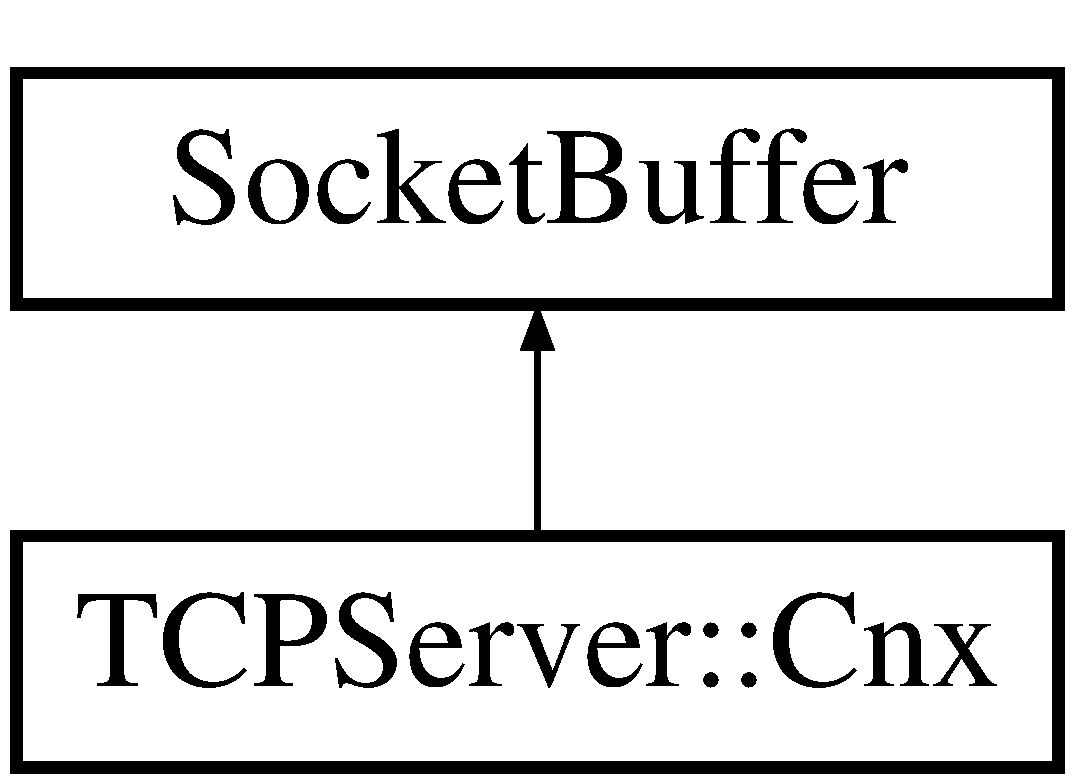
\includegraphics[height=2.000000cm]{classTCPServer_1_1Cnx}
\end{center}
\end{figure}
\subsection*{Public Member Functions}
\begin{DoxyCompactItemize}
\item 
\hypertarget{classTCPServer_1_1Cnx_affe5198f5dca75da9f651e286a289b47}{\hyperlink{classTCPServer}{T\-C\-P\-Server} $\ast$ {\bfseries server} ()}\label{classTCPServer_1_1Cnx_affe5198f5dca75da9f651e286a289b47}

\item 
\hypertarget{classTCPServer_1_1Cnx_a3dd1fff38f6463d62ef5f3cae4fad340}{pthread\-\_\-t {\bfseries thread} ()}\label{classTCPServer_1_1Cnx_a3dd1fff38f6463d62ef5f3cae4fad340}

\end{DoxyCompactItemize}
\subsection*{Friends}
\begin{DoxyCompactItemize}
\item 
\hypertarget{classTCPServer_1_1Cnx_ae4cfdb1814d91a8d28dadb49adda68f0}{class {\bfseries T\-C\-P\-Server}}\label{classTCPServer_1_1Cnx_ae4cfdb1814d91a8d28dadb49adda68f0}

\end{DoxyCompactItemize}
\subsection*{Additional Inherited Members}


\subsection{Detailed Description}
represents a connection with a given client. 

The documentation for this class was generated from the following files\-:\begin{DoxyCompactItemize}
\item 
T\-C\-P\-Server.\-h\item 
T\-C\-P\-Server.\-cpp\end{DoxyCompactItemize}

\hypertarget{classFilm}{\section{Film Class Reference}
\label{classFilm}\index{Film@{Film}}
}


The \hyperlink{classFilm}{Film} class params\-: count\-: unsigned int $\ast$durees\-: unsigned int methods\-: \hyperlink{classFilm_acf9c4384117b17333e434d410914d48b}{set\-Durees(unsigned int $\ast$tab, unsigned int num)} \hyperlink{classFilm_a2beb91b3aa53d2b1f25e43783585aaf0}{get\-Durees()} \hyperlink{classFilm_a094ff01cf9629b9ec0bed4e6efd140d3}{get\-Nombre\-Chapitres()} \hyperlink{classFilm_a0fd2b4ba12627d9268fb0ee64b850b15}{affichage(ostream \& s)}  




{\ttfamily \#include $<$film.\-h$>$}

Inheritance diagram for Film\-:\begin{figure}[H]
\begin{center}
\leavevmode
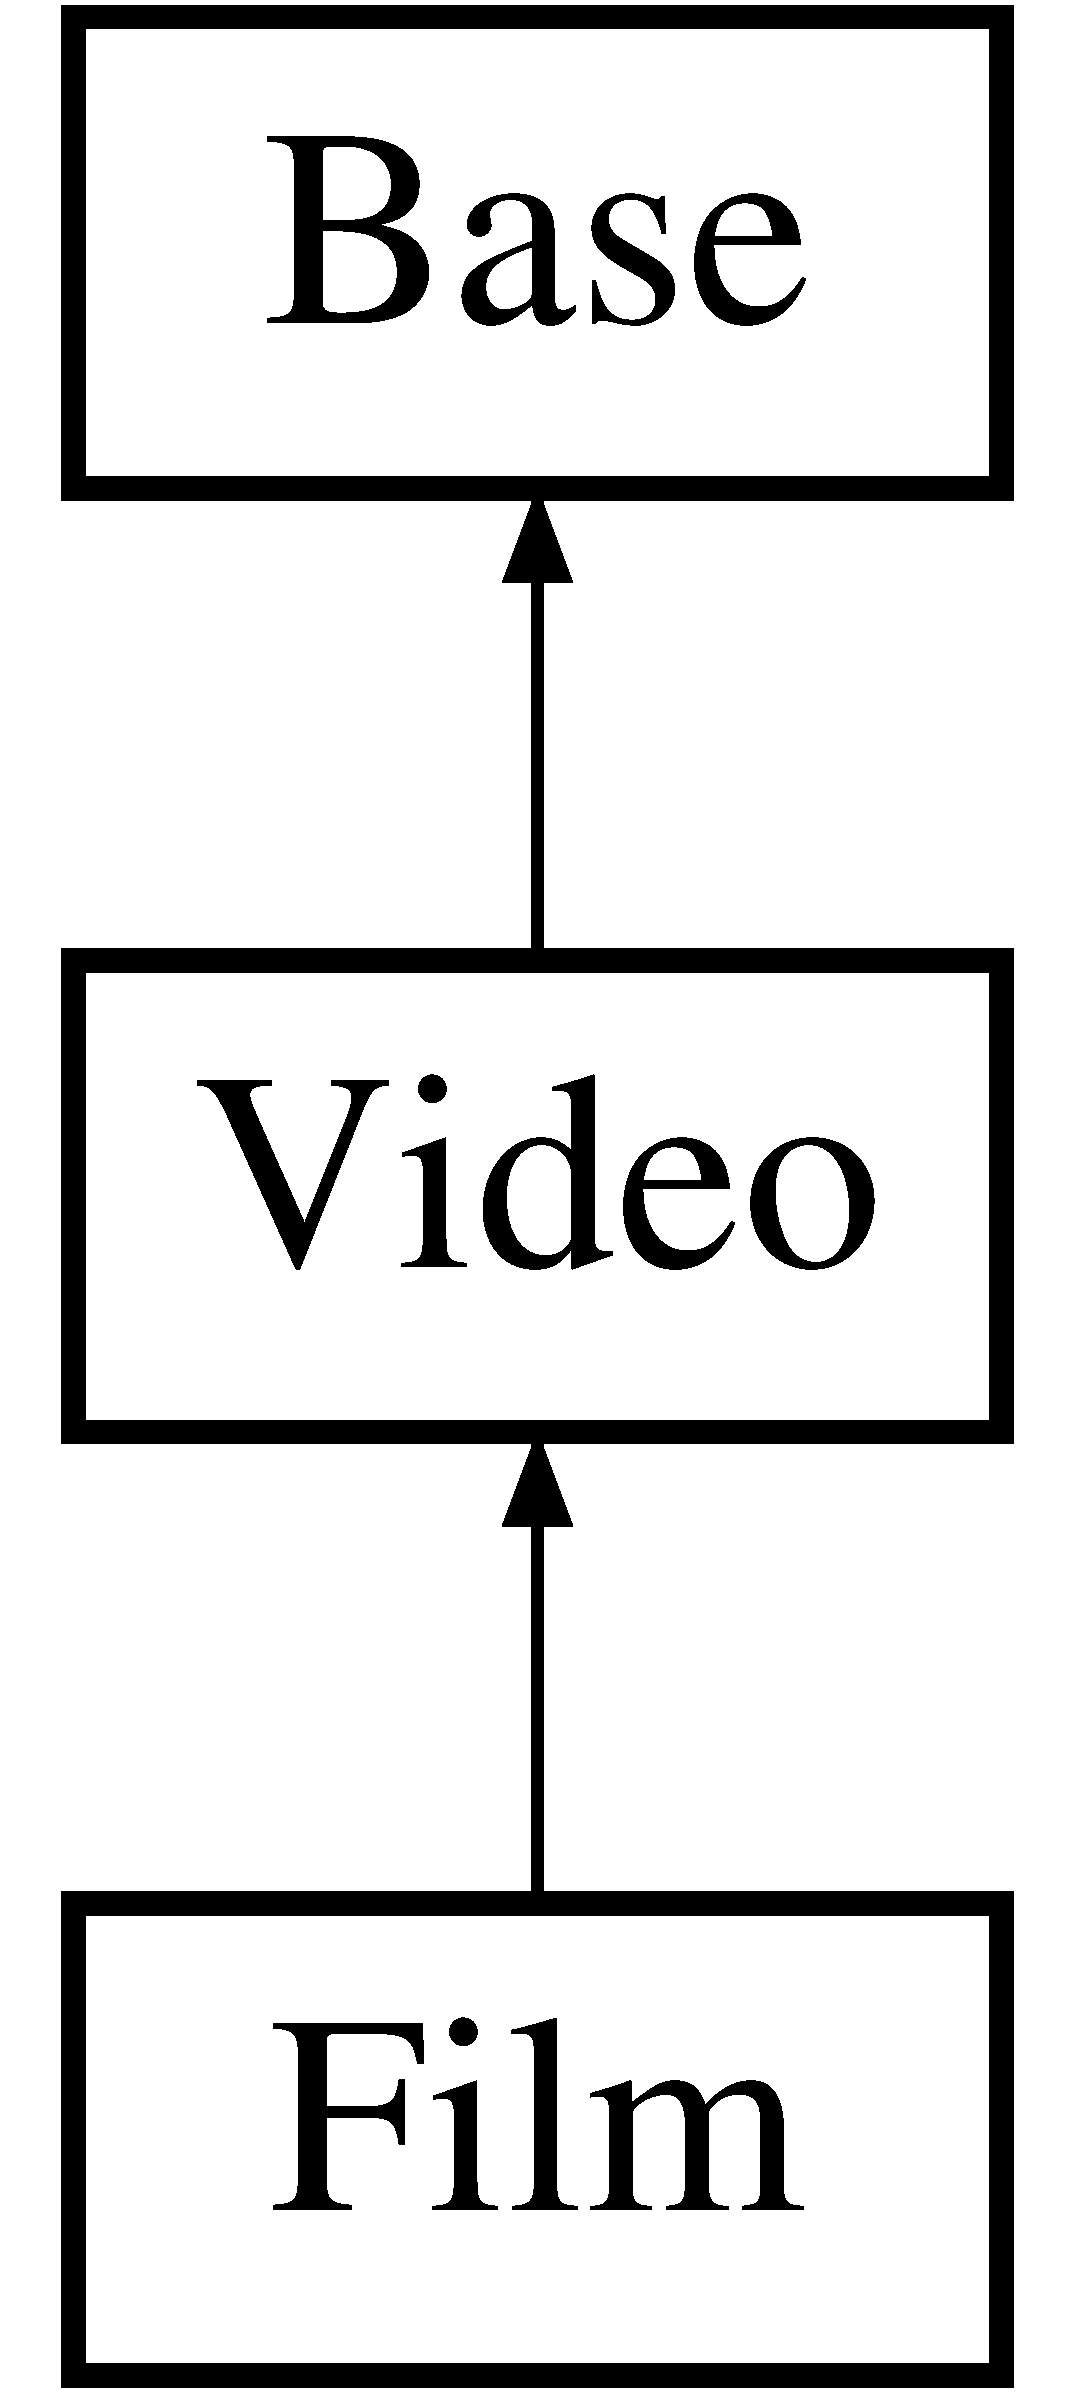
\includegraphics[height=3.000000cm]{classFilm}
\end{center}
\end{figure}
\subsection*{Public Member Functions}
\begin{DoxyCompactItemize}
\item 
\hypertarget{classFilm_af2835db2b0ef3a87aaa3222f4d9d1ae3}{\hyperlink{classFilm_af2835db2b0ef3a87aaa3222f4d9d1ae3}{Film} ()}\label{classFilm_af2835db2b0ef3a87aaa3222f4d9d1ae3}

\begin{DoxyCompactList}\small\item\em \hyperlink{classFilm}{Film} constructor overcharge. \end{DoxyCompactList}\item 
\hyperlink{classFilm_a9d262bf64fd6de5a6f272ed75bae4dba}{Film} (string name, string pathname, int duree)
\begin{DoxyCompactList}\small\item\em \hyperlink{classFilm}{Film} Constructor. \end{DoxyCompactList}\item 
virtual void \hyperlink{classFilm_acf9c4384117b17333e434d410914d48b}{set\-Durees} (unsigned int $\ast$tab, unsigned int num)
\begin{DoxyCompactList}\small\item\em set\-Durees \end{DoxyCompactList}\item 
virtual unsigned const int $\ast$ \hyperlink{classFilm_a2beb91b3aa53d2b1f25e43783585aaf0}{get\-Durees} () const 
\begin{DoxyCompactList}\small\item\em get\-Durees \end{DoxyCompactList}\item 
virtual int \hyperlink{classFilm_a094ff01cf9629b9ec0bed4e6efd140d3}{get\-Nombre\-Chapitres} () const 
\begin{DoxyCompactList}\small\item\em get\-Nombre\-Chapitres \end{DoxyCompactList}\item 
virtual string \hyperlink{classFilm_a0fd2b4ba12627d9268fb0ee64b850b15}{affichage} (ostream \&s) override
\begin{DoxyCompactList}\small\item\em affichage \end{DoxyCompactList}\item 
\hypertarget{classFilm_a490465154daeb29961fddb843a864eeb}{virtual \hyperlink{classFilm_a490465154daeb29961fddb843a864eeb}{$\sim$\-Film} ()}\label{classFilm_a490465154daeb29961fddb843a864eeb}

\begin{DoxyCompactList}\small\item\em $\sim$\-Film Destructor \end{DoxyCompactList}\end{DoxyCompactItemize}


\subsection{Detailed Description}
The \hyperlink{classFilm}{Film} class params\-: count\-: unsigned int $\ast$durees\-: unsigned int methods\-: \hyperlink{classFilm_acf9c4384117b17333e434d410914d48b}{set\-Durees(unsigned int $\ast$tab, unsigned int num)} \hyperlink{classFilm_a2beb91b3aa53d2b1f25e43783585aaf0}{get\-Durees()} \hyperlink{classFilm_a094ff01cf9629b9ec0bed4e6efd140d3}{get\-Nombre\-Chapitres()} \hyperlink{classFilm_a0fd2b4ba12627d9268fb0ee64b850b15}{affichage(ostream \& s)} 

\subsection{Constructor \& Destructor Documentation}
\hypertarget{classFilm_a9d262bf64fd6de5a6f272ed75bae4dba}{\index{Film@{Film}!Film@{Film}}
\index{Film@{Film}!Film@{Film}}
\subsubsection[{Film}]{\setlength{\rightskip}{0pt plus 5cm}Film\-::\-Film (
\begin{DoxyParamCaption}
\item[{string}]{name, }
\item[{string}]{pathname, }
\item[{int}]{duree}
\end{DoxyParamCaption}
)\hspace{0.3cm}{\ttfamily [inline]}}}\label{classFilm_a9d262bf64fd6de5a6f272ed75bae4dba}


\hyperlink{classFilm}{Film} Constructor. 


\begin{DoxyParams}{Parameters}
{\em name} & string \\
\hline
{\em pathname} & string \\
\hline
{\em duree} & int Creates a film with the same parameters as a video \\
\hline
\end{DoxyParams}


\subsection{Member Function Documentation}
\hypertarget{classFilm_a0fd2b4ba12627d9268fb0ee64b850b15}{\index{Film@{Film}!affichage@{affichage}}
\index{affichage@{affichage}!Film@{Film}}
\subsubsection[{affichage}]{\setlength{\rightskip}{0pt plus 5cm}virtual string Film\-::affichage (
\begin{DoxyParamCaption}
\item[{ostream \&}]{s}
\end{DoxyParamCaption}
)\hspace{0.3cm}{\ttfamily [inline]}, {\ttfamily [override]}, {\ttfamily [virtual]}}}\label{classFilm_a0fd2b4ba12627d9268fb0ee64b850b15}


affichage 


\begin{DoxyParams}{Parameters}
{\em s} & ostream \\
\hline
\end{DoxyParams}
\begin{DoxyReturn}{Returns}
string of film attributes Also prints in s the return string 
\end{DoxyReturn}


Reimplemented from \hyperlink{classVideo_a180c985ff368f77d0fb66ec106106f00}{Video}.

\hypertarget{classFilm_a2beb91b3aa53d2b1f25e43783585aaf0}{\index{Film@{Film}!get\-Durees@{get\-Durees}}
\index{get\-Durees@{get\-Durees}!Film@{Film}}
\subsubsection[{get\-Durees}]{\setlength{\rightskip}{0pt plus 5cm}virtual unsigned const int$\ast$ Film\-::get\-Durees (
\begin{DoxyParamCaption}
{}
\end{DoxyParamCaption}
) const\hspace{0.3cm}{\ttfamily [inline]}, {\ttfamily [virtual]}}}\label{classFilm_a2beb91b3aa53d2b1f25e43783585aaf0}


get\-Durees 

\begin{DoxyReturn}{Returns}
pointer to array of durees 
\end{DoxyReturn}
\hypertarget{classFilm_a094ff01cf9629b9ec0bed4e6efd140d3}{\index{Film@{Film}!get\-Nombre\-Chapitres@{get\-Nombre\-Chapitres}}
\index{get\-Nombre\-Chapitres@{get\-Nombre\-Chapitres}!Film@{Film}}
\subsubsection[{get\-Nombre\-Chapitres}]{\setlength{\rightskip}{0pt plus 5cm}virtual int Film\-::get\-Nombre\-Chapitres (
\begin{DoxyParamCaption}
{}
\end{DoxyParamCaption}
) const\hspace{0.3cm}{\ttfamily [inline]}, {\ttfamily [virtual]}}}\label{classFilm_a094ff01cf9629b9ec0bed4e6efd140d3}


get\-Nombre\-Chapitres 

\begin{DoxyReturn}{Returns}
count\-: number of chapters 
\end{DoxyReturn}
\hypertarget{classFilm_acf9c4384117b17333e434d410914d48b}{\index{Film@{Film}!set\-Durees@{set\-Durees}}
\index{set\-Durees@{set\-Durees}!Film@{Film}}
\subsubsection[{set\-Durees}]{\setlength{\rightskip}{0pt plus 5cm}virtual void Film\-::set\-Durees (
\begin{DoxyParamCaption}
\item[{unsigned int $\ast$}]{tab, }
\item[{unsigned int}]{num}
\end{DoxyParamCaption}
)\hspace{0.3cm}{\ttfamily [inline]}, {\ttfamily [virtual]}}}\label{classFilm_acf9c4384117b17333e434d410914d48b}


set\-Durees 


\begin{DoxyParams}{Parameters}
{\em tab} & unsigned int \\
\hline
{\em num} & unsigned int Sets the parameter durees to the film, copying the variable tab to durees. \\
\hline
\end{DoxyParams}


The documentation for this class was generated from the following file\-:\begin{DoxyCompactItemize}
\item 
film.\-h\end{DoxyCompactItemize}

\hypertarget{classGroup}{\section{Group Class Reference}
\label{classGroup}\index{Group@{Group}}
}


The \hyperlink{classGroup}{Group} class params\-: name\-: string methods\-: \hyperlink{classGroup_a0c38a3d735a6bef446c1dceb27866408}{set\-Name(string n)} \hyperlink{classGroup_a030dc7b666d67a51926d6236c1707f14}{get\-Group\-Name()} \hyperlink{classGroup_ae5bd44de2616138eacca19189be39d3c}{affichage(ostream \& s)}  




{\ttfamily \#include $<$group.\-h$>$}

Inheritance diagram for Group\-:\begin{figure}[H]
\begin{center}
\leavevmode
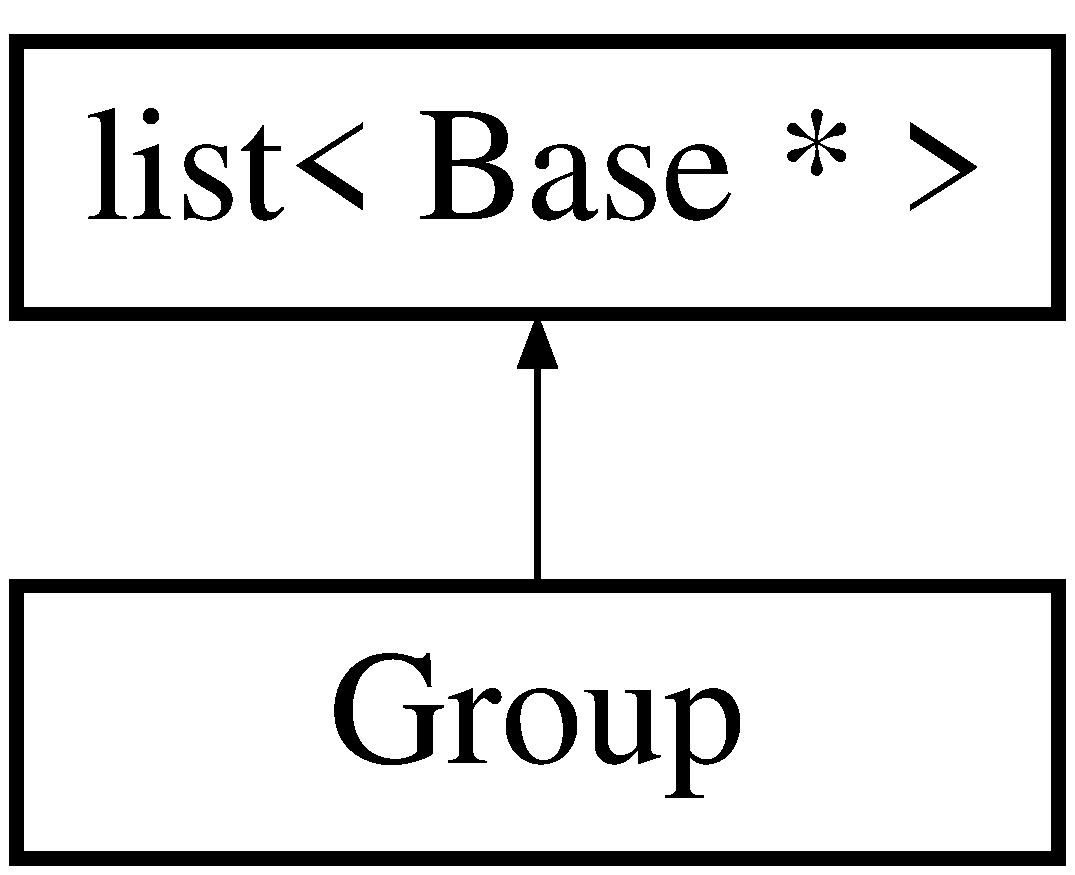
\includegraphics[height=2.000000cm]{classGroup}
\end{center}
\end{figure}
\subsection*{Public Member Functions}
\begin{DoxyCompactItemize}
\item 
\hypertarget{classGroup_a7b74f9ac68e0504ccf2e2854b7355ff1}{\hyperlink{classGroup_a7b74f9ac68e0504ccf2e2854b7355ff1}{Group} ()}\label{classGroup_a7b74f9ac68e0504ccf2e2854b7355ff1}

\begin{DoxyCompactList}\small\item\em \hyperlink{classGroup}{Group} Constructor overcharge. \end{DoxyCompactList}\item 
\hyperlink{classGroup_af214c730661c4bb60beb522c9e727539}{Group} (string name)
\begin{DoxyCompactList}\small\item\em \hyperlink{classGroup}{Group}. \end{DoxyCompactList}\item 
virtual void \hyperlink{classGroup_a0c38a3d735a6bef446c1dceb27866408}{set\-Name} (string n)
\begin{DoxyCompactList}\small\item\em set\-Name \end{DoxyCompactList}\item 
virtual string \hyperlink{classGroup_a030dc7b666d67a51926d6236c1707f14}{get\-Group\-Name} ()
\begin{DoxyCompactList}\small\item\em get\-Group\-Name \end{DoxyCompactList}\item 
virtual string \hyperlink{classGroup_ae5bd44de2616138eacca19189be39d3c}{affichage} (ostream \&s)
\begin{DoxyCompactList}\small\item\em affichage \end{DoxyCompactList}\item 
\hypertarget{classGroup_ad21d9df83f85ecd5c8ce51715d9c7456}{virtual \hyperlink{classGroup_ad21d9df83f85ecd5c8ce51715d9c7456}{$\sim$\-Group} ()}\label{classGroup_ad21d9df83f85ecd5c8ce51715d9c7456}

\begin{DoxyCompactList}\small\item\em $\sim$\-Group Destructor \end{DoxyCompactList}\end{DoxyCompactItemize}


\subsection{Detailed Description}
The \hyperlink{classGroup}{Group} class params\-: name\-: string methods\-: \hyperlink{classGroup_a0c38a3d735a6bef446c1dceb27866408}{set\-Name(string n)} \hyperlink{classGroup_a030dc7b666d67a51926d6236c1707f14}{get\-Group\-Name()} \hyperlink{classGroup_ae5bd44de2616138eacca19189be39d3c}{affichage(ostream \& s)} 

\subsection{Constructor \& Destructor Documentation}
\hypertarget{classGroup_af214c730661c4bb60beb522c9e727539}{\index{Group@{Group}!Group@{Group}}
\index{Group@{Group}!Group@{Group}}
\subsubsection[{Group}]{\setlength{\rightskip}{0pt plus 5cm}Group\-::\-Group (
\begin{DoxyParamCaption}
\item[{string}]{name}
\end{DoxyParamCaption}
)\hspace{0.3cm}{\ttfamily [inline]}}}\label{classGroup_af214c730661c4bb60beb522c9e727539}


\hyperlink{classGroup}{Group}. 


\begin{DoxyParams}{Parameters}
{\em name} & string \\
\hline
\end{DoxyParams}


\subsection{Member Function Documentation}
\hypertarget{classGroup_ae5bd44de2616138eacca19189be39d3c}{\index{Group@{Group}!affichage@{affichage}}
\index{affichage@{affichage}!Group@{Group}}
\subsubsection[{affichage}]{\setlength{\rightskip}{0pt plus 5cm}virtual string Group\-::affichage (
\begin{DoxyParamCaption}
\item[{ostream \&}]{s}
\end{DoxyParamCaption}
)\hspace{0.3cm}{\ttfamily [inline]}, {\ttfamily [virtual]}}}\label{classGroup_ae5bd44de2616138eacca19189be39d3c}


affichage 


\begin{DoxyParams}{Parameters}
{\em s} & ostream \\
\hline
\end{DoxyParams}
\begin{DoxyReturn}{Returns}
string of attributes of group Prints through s the returned string 
\end{DoxyReturn}
\hypertarget{classGroup_a030dc7b666d67a51926d6236c1707f14}{\index{Group@{Group}!get\-Group\-Name@{get\-Group\-Name}}
\index{get\-Group\-Name@{get\-Group\-Name}!Group@{Group}}
\subsubsection[{get\-Group\-Name}]{\setlength{\rightskip}{0pt plus 5cm}virtual string Group\-::get\-Group\-Name (
\begin{DoxyParamCaption}
{}
\end{DoxyParamCaption}
)\hspace{0.3cm}{\ttfamily [inline]}, {\ttfamily [virtual]}}}\label{classGroup_a030dc7b666d67a51926d6236c1707f14}


get\-Group\-Name 

\begin{DoxyReturn}{Returns}
string of group name 
\end{DoxyReturn}
\hypertarget{classGroup_a0c38a3d735a6bef446c1dceb27866408}{\index{Group@{Group}!set\-Name@{set\-Name}}
\index{set\-Name@{set\-Name}!Group@{Group}}
\subsubsection[{set\-Name}]{\setlength{\rightskip}{0pt plus 5cm}virtual void Group\-::set\-Name (
\begin{DoxyParamCaption}
\item[{string}]{n}
\end{DoxyParamCaption}
)\hspace{0.3cm}{\ttfamily [inline]}, {\ttfamily [virtual]}}}\label{classGroup_a0c38a3d735a6bef446c1dceb27866408}


set\-Name 


\begin{DoxyParams}{Parameters}
{\em n} & string Sets the name of the group to n \\
\hline
\end{DoxyParams}


The documentation for this class was generated from the following file\-:\begin{DoxyCompactItemize}
\item 
group.\-h\end{DoxyCompactItemize}

\hypertarget{structInputBuffer}{\section{Input\-Buffer Struct Reference}
\label{structInputBuffer}\index{Input\-Buffer@{Input\-Buffer}}
}
\subsection*{Public Member Functions}
\begin{DoxyCompactItemize}
\item 
\hypertarget{structInputBuffer_a9409ec8e4581caa99dcac1af963349b5}{{\bfseries Input\-Buffer} (size\-\_\-t size)}\label{structInputBuffer_a9409ec8e4581caa99dcac1af963349b5}

\end{DoxyCompactItemize}
\subsection*{Public Attributes}
\begin{DoxyCompactItemize}
\item 
\hypertarget{structInputBuffer_aee7a717b6cf023deabe9910410e6cfb6}{char $\ast$ {\bfseries buffer}}\label{structInputBuffer_aee7a717b6cf023deabe9910410e6cfb6}

\item 
\hypertarget{structInputBuffer_a2f05121c4fb8571845cc22d083c6da46}{char $\ast$ {\bfseries begin}}\label{structInputBuffer_a2f05121c4fb8571845cc22d083c6da46}

\item 
\hypertarget{structInputBuffer_a52ba71c71b9b955b8369fc5217e3c4b6}{char $\ast$ {\bfseries end}}\label{structInputBuffer_a52ba71c71b9b955b8369fc5217e3c4b6}

\item 
\hypertarget{structInputBuffer_a621d633184a77c449e7b07d705870ae2}{ssize\-\_\-t {\bfseries remaining}}\label{structInputBuffer_a621d633184a77c449e7b07d705870ae2}

\end{DoxyCompactItemize}


The documentation for this struct was generated from the following file\-:\begin{DoxyCompactItemize}
\item 
Socket.\-cpp\end{DoxyCompactItemize}

\hypertarget{classInvalidCaracters}{\section{Invalid\-Caracters Class Reference}
\label{classInvalidCaracters}\index{Invalid\-Caracters@{Invalid\-Caracters}}
}
Inheritance diagram for Invalid\-Caracters\-:\begin{figure}[H]
\begin{center}
\leavevmode
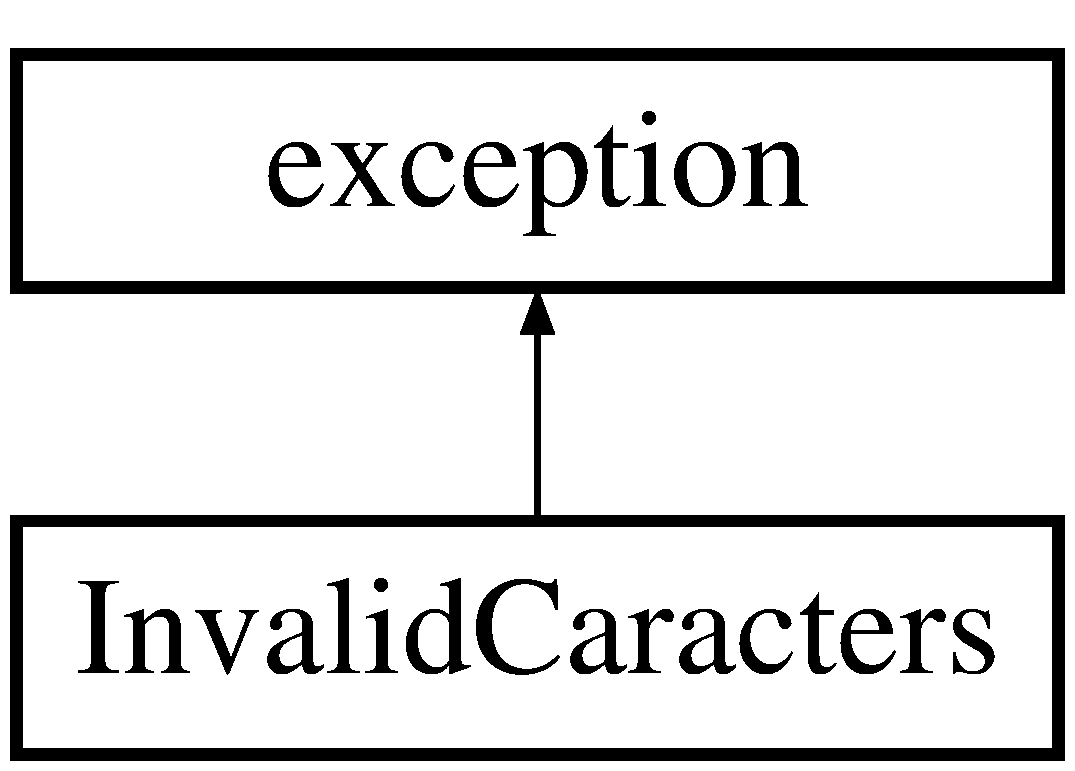
\includegraphics[height=2.000000cm]{classInvalidCaracters}
\end{center}
\end{figure}


\subsection{Detailed Description}
Exception \hyperlink{classInvalidCaracters}{Invalid\-Caracters} that will be launched if there are any special characters 

The documentation for this class was generated from the following file\-:\begin{DoxyCompactItemize}
\item 
catalogue.\-cpp\end{DoxyCompactItemize}

\hypertarget{classTCPServer_1_1Lock}{\section{T\-C\-P\-Server\-:\-:Lock Class Reference}
\label{classTCPServer_1_1Lock}\index{T\-C\-P\-Server\-::\-Lock@{T\-C\-P\-Server\-::\-Lock}}
}


locks the server in read mode or in write mode. In order to avoid concurrency problems between threads, the callback method that processes requests should instantiate a \hyperlink{classTCPServer_1_1Lock}{Lock} object in the stack. The \hyperlink{classTCPServer_1_1Lock}{Lock} must be instantiated in write mode if the request changes data, or in read mode otherwise. A write lock blocks all other locks (hence, all other threads) until the callback method that issued the write lock returns.  




{\ttfamily \#include $<$T\-C\-P\-Server.\-h$>$}

\subsection*{Public Member Functions}
\begin{DoxyCompactItemize}
\item 
\hypertarget{classTCPServer_1_1Lock_a4b1fa591dde407aacd93133828cfac81}{\hyperlink{classTCPServer_1_1Lock_a4b1fa591dde407aacd93133828cfac81}{Lock} (\hyperlink{classTCPServer_1_1Cnx}{Cnx} \&, bool write\-Mode=false)}\label{classTCPServer_1_1Lock_a4b1fa591dde407aacd93133828cfac81}

\begin{DoxyCompactList}\small\item\em locks the connection in write mode if the second argument is true and in read mode otherwise. \end{DoxyCompactList}\end{DoxyCompactItemize}


\subsection{Detailed Description}
locks the server in read mode or in write mode. In order to avoid concurrency problems between threads, the callback method that processes requests should instantiate a \hyperlink{classTCPServer_1_1Lock}{Lock} object in the stack. The \hyperlink{classTCPServer_1_1Lock}{Lock} must be instantiated in write mode if the request changes data, or in read mode otherwise. A write lock blocks all other locks (hence, all other threads) until the callback method that issued the write lock returns. 

The documentation for this class was generated from the following files\-:\begin{DoxyCompactItemize}
\item 
T\-C\-P\-Server.\-h\item 
T\-C\-P\-Server.\-cpp\end{DoxyCompactItemize}

\hypertarget{classMyApp}{\section{My\-App Class Reference}
\label{classMyApp}\index{My\-App@{My\-App}}
}
\subsection*{Public Member Functions}
\begin{DoxyCompactItemize}
\item 
bool \hyperlink{classMyApp_a206ebe9c95c740b7104bb866844b8dcd}{process\-Request} (\hyperlink{classTCPServer_1_1Cnx}{T\-C\-P\-Server\-::\-Cnx} \&cnx, const string \&request, string \&response)
\item 
bool \hyperlink{classMyApp_a206ebe9c95c740b7104bb866844b8dcd}{process\-Request} (\hyperlink{classTCPServer_1_1Cnx}{T\-C\-P\-Server\-::\-Cnx} \&cnx, const string \&request, string \&response)
\end{DoxyCompactItemize}


\subsection{Member Function Documentation}
\hypertarget{classMyApp_a206ebe9c95c740b7104bb866844b8dcd}{\index{My\-App@{My\-App}!process\-Request@{process\-Request}}
\index{process\-Request@{process\-Request}!MyApp@{My\-App}}
\subsubsection[{process\-Request}]{\setlength{\rightskip}{0pt plus 5cm}bool My\-App\-::process\-Request (
\begin{DoxyParamCaption}
\item[{{\bf T\-C\-P\-Server\-::\-Cnx} \&}]{cnx, }
\item[{const string \&}]{request, }
\item[{string \&}]{response}
\end{DoxyParamCaption}
)\hspace{0.3cm}{\ttfamily [inline]}}}\label{classMyApp_a206ebe9c95c740b7104bb866844b8dcd}
Cette fonction est appelée chaque fois qu'il y a une requête à traiter.
\begin{DoxyItemize}
\item 'request' contient la requête
\item 'response' sert à indiquer la réponse qui sera renvoyée au client
\item si la fonction renvoie false la connexion est close. 
\end{DoxyItemize}Creates new catalogue with default parameters photo\-: disney.\-jpg video\-: video1.\-mp4 film\-: film

If the petition has \char`\"{}rechercher\char`\"{} or \char`\"{}1\char`\"{} followed by a multimedia object name the client will receive the answer for the method rechercher\-Multimedia

If the petition has \char`\"{}jouer\char`\"{} or \char`\"{}2\char`\"{} followed by a multimedia object name, the server will open the object and alert the client that it is being played \hypertarget{classMyApp_a206ebe9c95c740b7104bb866844b8dcd}{\index{My\-App@{My\-App}!process\-Request@{process\-Request}}
\index{process\-Request@{process\-Request}!MyApp@{My\-App}}
\subsubsection[{process\-Request}]{\setlength{\rightskip}{0pt plus 5cm}bool My\-App\-::process\-Request (
\begin{DoxyParamCaption}
\item[{{\bf T\-C\-P\-Server\-::\-Cnx} \&}]{cnx, }
\item[{const string \&}]{request, }
\item[{string \&}]{response}
\end{DoxyParamCaption}
)\hspace{0.3cm}{\ttfamily [inline]}}}\label{classMyApp_a206ebe9c95c740b7104bb866844b8dcd}
Cette fonction est appelée chaque fois qu'il y a une requête à traiter.
\begin{DoxyItemize}
\item 'request' contient la requête
\item 'response' sert à indiquer la réponse qui sera renvoyée au client
\item si la fonction renvoie false la connexion est close. 
\end{DoxyItemize}

The documentation for this class was generated from the following files\-:\begin{DoxyCompactItemize}
\item 
server.\-cpp\item 
servercatalogue.\-cpp\end{DoxyCompactItemize}

\hypertarget{classPhoto}{\section{Photo Class Reference}
\label{classPhoto}\index{Photo@{Photo}}
}


The \hyperlink{classPhoto}{Photo} class params\-: lat\-: double lon\-: double methods\-: \hyperlink{classPhoto_a2a33bfd34dc606f17f4cb4ff1505afbe}{set\-Latitude(double la)} \hyperlink{classPhoto_a5846dcbc510174ed2db5cbbe99367a7f}{set\-Longitude(double lo)} \hyperlink{classPhoto_ac96f7a44787994f828e1fb24a4bdf768}{get\-Latitude()} \hyperlink{classPhoto_a736b26be1028d360f59800512b89b287}{get\-Longitude()} \hyperlink{classPhoto_a37b62ddde8114037efc2f8a8e97d0df0}{open\-Object()} \hyperlink{classPhoto_a2965c65d2ad33ebf2ac3b3cfad123fbb}{affichage(ostream \&s)}  




{\ttfamily \#include $<$photo.\-h$>$}

Inheritance diagram for Photo\-:\begin{figure}[H]
\begin{center}
\leavevmode
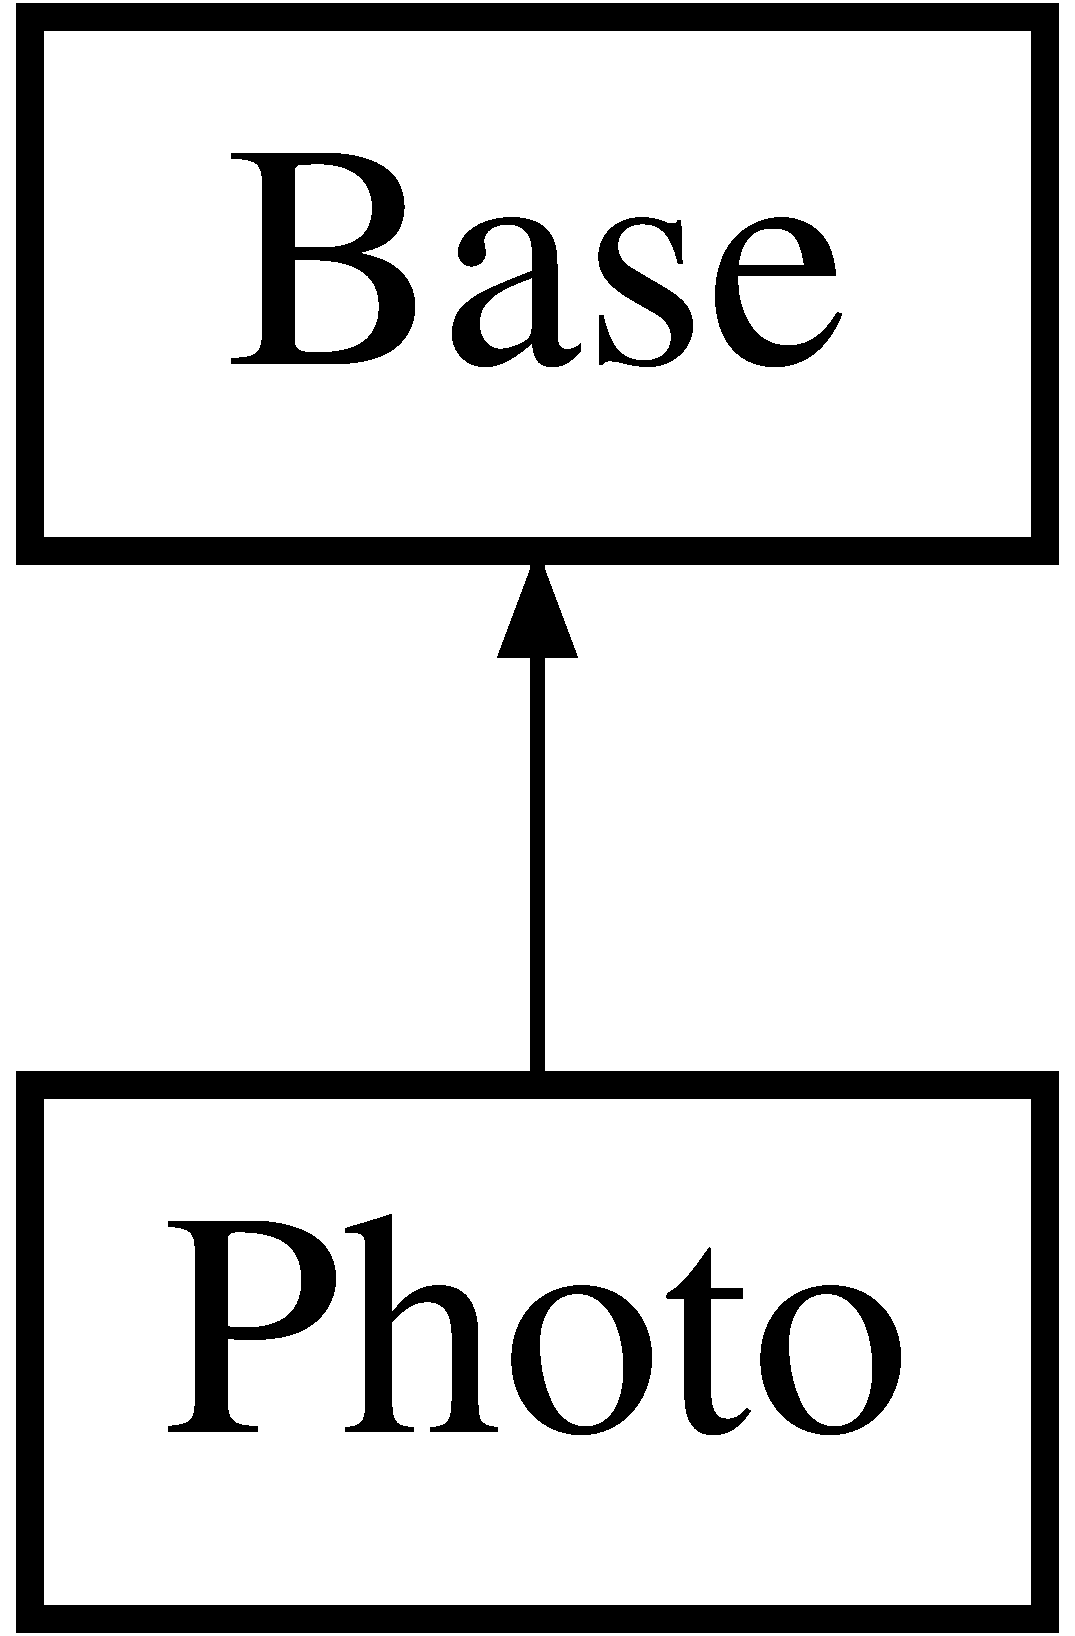
\includegraphics[height=2.000000cm]{classPhoto}
\end{center}
\end{figure}
\subsection*{Public Member Functions}
\begin{DoxyCompactItemize}
\item 
\hypertarget{classPhoto_a10ef03ede9235052eb9f7d5e950f85d3}{\hyperlink{classPhoto_a10ef03ede9235052eb9f7d5e950f85d3}{Photo} ()}\label{classPhoto_a10ef03ede9235052eb9f7d5e950f85d3}

\begin{DoxyCompactList}\small\item\em \hyperlink{classPhoto}{Photo} Constructor Overcharge. \end{DoxyCompactList}\item 
\hyperlink{classPhoto_a6f5de7ca78d5a4b10ce8b5e86c346452}{Photo} (string name, string pathname, double lat, double lon)
\begin{DoxyCompactList}\small\item\em \hyperlink{classPhoto}{Photo}. \end{DoxyCompactList}\item 
virtual void \hyperlink{classPhoto_a2a33bfd34dc606f17f4cb4ff1505afbe}{set\-Latitude} (double la)
\begin{DoxyCompactList}\small\item\em set\-Latitude \end{DoxyCompactList}\item 
virtual void \hyperlink{classPhoto_a5846dcbc510174ed2db5cbbe99367a7f}{set\-Longitude} (double lo)
\begin{DoxyCompactList}\small\item\em set\-Longitude \end{DoxyCompactList}\item 
virtual int \hyperlink{classPhoto_ac96f7a44787994f828e1fb24a4bdf768}{get\-Latitude} () const 
\begin{DoxyCompactList}\small\item\em get\-Latitude \end{DoxyCompactList}\item 
virtual int \hyperlink{classPhoto_a736b26be1028d360f59800512b89b287}{get\-Longitude} () const 
\begin{DoxyCompactList}\small\item\em get\-Longitude \end{DoxyCompactList}\item 
\hypertarget{classPhoto_a37b62ddde8114037efc2f8a8e97d0df0}{virtual void \hyperlink{classPhoto_a37b62ddde8114037efc2f8a8e97d0df0}{open\-Object} ()}\label{classPhoto_a37b62ddde8114037efc2f8a8e97d0df0}

\begin{DoxyCompactList}\small\item\em open\-Object Opens image with xdg-\/open (default program) due to the fact that with imagej, it would not work properly without the \char`\"{}\&\char`\"{}, and this solution worked better \end{DoxyCompactList}\item 
virtual string \hyperlink{classPhoto_a2965c65d2ad33ebf2ac3b3cfad123fbb}{affichage} (ostream \&s) override
\begin{DoxyCompactList}\small\item\em affichage \end{DoxyCompactList}\item 
\hypertarget{classPhoto_a1bf707fc71f95a3aa3464bd4e339afd0}{virtual \hyperlink{classPhoto_a1bf707fc71f95a3aa3464bd4e339afd0}{$\sim$\-Photo} ()}\label{classPhoto_a1bf707fc71f95a3aa3464bd4e339afd0}

\begin{DoxyCompactList}\small\item\em $\sim$\-Photo Destructor \end{DoxyCompactList}\end{DoxyCompactItemize}


\subsection{Detailed Description}
The \hyperlink{classPhoto}{Photo} class params\-: lat\-: double lon\-: double methods\-: \hyperlink{classPhoto_a2a33bfd34dc606f17f4cb4ff1505afbe}{set\-Latitude(double la)} \hyperlink{classPhoto_a5846dcbc510174ed2db5cbbe99367a7f}{set\-Longitude(double lo)} \hyperlink{classPhoto_ac96f7a44787994f828e1fb24a4bdf768}{get\-Latitude()} \hyperlink{classPhoto_a736b26be1028d360f59800512b89b287}{get\-Longitude()} \hyperlink{classPhoto_a37b62ddde8114037efc2f8a8e97d0df0}{open\-Object()} \hyperlink{classPhoto_a2965c65d2ad33ebf2ac3b3cfad123fbb}{affichage(ostream \&s)} 

\subsection{Constructor \& Destructor Documentation}
\hypertarget{classPhoto_a6f5de7ca78d5a4b10ce8b5e86c346452}{\index{Photo@{Photo}!Photo@{Photo}}
\index{Photo@{Photo}!Photo@{Photo}}
\subsubsection[{Photo}]{\setlength{\rightskip}{0pt plus 5cm}Photo\-::\-Photo (
\begin{DoxyParamCaption}
\item[{string}]{name, }
\item[{string}]{pathname, }
\item[{double}]{lat, }
\item[{double}]{lon}
\end{DoxyParamCaption}
)\hspace{0.3cm}{\ttfamily [inline]}}}\label{classPhoto_a6f5de7ca78d5a4b10ce8b5e86c346452}


\hyperlink{classPhoto}{Photo}. 


\begin{DoxyParams}{Parameters}
{\em name} & string \\
\hline
{\em pathname} & string \\
\hline
{\em lat} & double \\
\hline
{\em lon} & double \\
\hline
\end{DoxyParams}


\subsection{Member Function Documentation}
\hypertarget{classPhoto_a2965c65d2ad33ebf2ac3b3cfad123fbb}{\index{Photo@{Photo}!affichage@{affichage}}
\index{affichage@{affichage}!Photo@{Photo}}
\subsubsection[{affichage}]{\setlength{\rightskip}{0pt plus 5cm}virtual string Photo\-::affichage (
\begin{DoxyParamCaption}
\item[{ostream \&}]{s}
\end{DoxyParamCaption}
)\hspace{0.3cm}{\ttfamily [inline]}, {\ttfamily [override]}, {\ttfamily [virtual]}}}\label{classPhoto_a2965c65d2ad33ebf2ac3b3cfad123fbb}


affichage 


\begin{DoxyParams}{Parameters}
{\em s} & ostream \\
\hline
\end{DoxyParams}
\begin{DoxyReturn}{Returns}
string of all photo attributes Prints through s the returned string 
\end{DoxyReturn}


Reimplemented from \hyperlink{classBase_ad712ff856464b0d3fa96d07eae70a90e}{Base}.

\hypertarget{classPhoto_ac96f7a44787994f828e1fb24a4bdf768}{\index{Photo@{Photo}!get\-Latitude@{get\-Latitude}}
\index{get\-Latitude@{get\-Latitude}!Photo@{Photo}}
\subsubsection[{get\-Latitude}]{\setlength{\rightskip}{0pt plus 5cm}virtual int Photo\-::get\-Latitude (
\begin{DoxyParamCaption}
{}
\end{DoxyParamCaption}
) const\hspace{0.3cm}{\ttfamily [inline]}, {\ttfamily [virtual]}}}\label{classPhoto_ac96f7a44787994f828e1fb24a4bdf768}


get\-Latitude 

\begin{DoxyReturn}{Returns}
lat double 
\end{DoxyReturn}
\hypertarget{classPhoto_a736b26be1028d360f59800512b89b287}{\index{Photo@{Photo}!get\-Longitude@{get\-Longitude}}
\index{get\-Longitude@{get\-Longitude}!Photo@{Photo}}
\subsubsection[{get\-Longitude}]{\setlength{\rightskip}{0pt plus 5cm}virtual int Photo\-::get\-Longitude (
\begin{DoxyParamCaption}
{}
\end{DoxyParamCaption}
) const\hspace{0.3cm}{\ttfamily [inline]}, {\ttfamily [virtual]}}}\label{classPhoto_a736b26be1028d360f59800512b89b287}


get\-Longitude 

\begin{DoxyReturn}{Returns}
lon double 
\end{DoxyReturn}
\hypertarget{classPhoto_a2a33bfd34dc606f17f4cb4ff1505afbe}{\index{Photo@{Photo}!set\-Latitude@{set\-Latitude}}
\index{set\-Latitude@{set\-Latitude}!Photo@{Photo}}
\subsubsection[{set\-Latitude}]{\setlength{\rightskip}{0pt plus 5cm}virtual void Photo\-::set\-Latitude (
\begin{DoxyParamCaption}
\item[{double}]{la}
\end{DoxyParamCaption}
)\hspace{0.3cm}{\ttfamily [inline]}, {\ttfamily [virtual]}}}\label{classPhoto_a2a33bfd34dc606f17f4cb4ff1505afbe}


set\-Latitude 


\begin{DoxyParams}{Parameters}
{\em la} & double sets lat to the value of la \\
\hline
\end{DoxyParams}
\hypertarget{classPhoto_a5846dcbc510174ed2db5cbbe99367a7f}{\index{Photo@{Photo}!set\-Longitude@{set\-Longitude}}
\index{set\-Longitude@{set\-Longitude}!Photo@{Photo}}
\subsubsection[{set\-Longitude}]{\setlength{\rightskip}{0pt plus 5cm}virtual void Photo\-::set\-Longitude (
\begin{DoxyParamCaption}
\item[{double}]{lo}
\end{DoxyParamCaption}
)\hspace{0.3cm}{\ttfamily [inline]}, {\ttfamily [virtual]}}}\label{classPhoto_a5846dcbc510174ed2db5cbbe99367a7f}


set\-Longitude 


\begin{DoxyParams}{Parameters}
{\em lo} & double sets lon to the value of lo \\
\hline
\end{DoxyParams}


The documentation for this class was generated from the following file\-:\begin{DoxyCompactItemize}
\item 
photo.\-h\end{DoxyCompactItemize}

\hypertarget{classServerSocket}{\section{Server\-Socket Class Reference}
\label{classServerSocket}\index{Server\-Socket@{Server\-Socket}}
}


T\-C\-P/\-I\-P \hyperlink{classSocket}{Socket} Server. This class encapsulates a T\-C\-P/\-I\-P socket server. A\-F\-\_\-\-I\-N\-E\-T connections following the I\-Pv4 Internet protocol are supported.  




{\ttfamily \#include $<$Socket.\-h$>$}

\subsection*{Public Member Functions}
\begin{DoxyCompactItemize}
\item 
\hypertarget{classServerSocket_a2b3098589541243241ca25495155186c}{\hyperlink{classServerSocket_a2b3098589541243241ca25495155186c}{Server\-Socket} ()}\label{classServerSocket_a2b3098589541243241ca25495155186c}

\begin{DoxyCompactList}\small\item\em Creates a new server socket. Creates a listening socket that waits for connection requests by T\-C\-P/\-I\-P clients. \end{DoxyCompactList}\item 
virtual \hyperlink{classSocket}{Socket} $\ast$ \hyperlink{classServerSocket_accc3d56d42aa50a5f3c920cf0b26959b}{accept} ()
\begin{DoxyCompactList}\small\item\em Accepts a new connection request and returns the corresponding socket. By default, this function blocks the caller until a connection is present. \end{DoxyCompactList}\item 
virtual int \hyperlink{classServerSocket_ad5281fe6c005bca007a9a758bd612481}{bind} (int port, int backlog=50)
\begin{DoxyCompactList}\small\item\em Assigns the socket to the local address. The socket must be bound before using it. \end{DoxyCompactList}\item 
\hypertarget{classServerSocket_a3eac6d5571bb092622d328dbda2de2cf}{virtual int \hyperlink{classServerSocket_a3eac6d5571bb092622d328dbda2de2cf}{close} ()}\label{classServerSocket_a3eac6d5571bb092622d328dbda2de2cf}

\begin{DoxyCompactList}\small\item\em Closes the socket. \end{DoxyCompactList}\item 
\hypertarget{classServerSocket_ad5b053b711f97cfe8b56f6febc15df65}{bool \hyperlink{classServerSocket_ad5b053b711f97cfe8b56f6febc15df65}{is\-Closed} () const }\label{classServerSocket_ad5b053b711f97cfe8b56f6febc15df65}

\begin{DoxyCompactList}\small\item\em Returns true if the socket has been closed. \end{DoxyCompactList}\item 
\hypertarget{classServerSocket_a57b5b84a60906153d9755190cdfd0d39}{int \hyperlink{classServerSocket_a57b5b84a60906153d9755190cdfd0d39}{descriptor} ()}\label{classServerSocket_a57b5b84a60906153d9755190cdfd0d39}

\begin{DoxyCompactList}\small\item\em Returns the Unix descriptor of the socket. \end{DoxyCompactList}\item 
\hypertarget{classServerSocket_ab34154bc6114c638ae02f5e018121099}{int \hyperlink{classServerSocket_ab34154bc6114c638ae02f5e018121099}{set\-Receive\-Buffer\-Size} (int size)}\label{classServerSocket_ab34154bc6114c638ae02f5e018121099}

\begin{DoxyCompactList}\small\item\em Sets the S\-O\-\_\-\-R\-C\-V\-B\-U\-F option to the specified value. \end{DoxyCompactList}\item 
\hypertarget{classServerSocket_ae60d7cc31ad535e5d3cac42e38b8ec98}{int \hyperlink{classServerSocket_ae60d7cc31ad535e5d3cac42e38b8ec98}{set\-Reuse\-Address} (bool)}\label{classServerSocket_ae60d7cc31ad535e5d3cac42e38b8ec98}

\begin{DoxyCompactList}\small\item\em Enables/disables the S\-O\-\_\-\-R\-E\-U\-S\-E\-A\-D\-D\-R socket option. \end{DoxyCompactList}\item 
\hypertarget{classServerSocket_aedb9144c9c375fcb14ac47bcb9d2eb17}{int \hyperlink{classServerSocket_aedb9144c9c375fcb14ac47bcb9d2eb17}{set\-So\-Timeout} (int timeout)}\label{classServerSocket_aedb9144c9c375fcb14ac47bcb9d2eb17}

\begin{DoxyCompactList}\small\item\em Enables/disables S\-O\-\_\-\-T\-I\-M\-E\-O\-U\-T with the specified timeout (in milliseconds). \end{DoxyCompactList}\item 
\hypertarget{classServerSocket_a9e5e1ee852ba26156c757a0086b780fe}{int \hyperlink{classServerSocket_a9e5e1ee852ba26156c757a0086b780fe}{set\-Tcp\-No\-Delay} (bool)}\label{classServerSocket_a9e5e1ee852ba26156c757a0086b780fe}

\begin{DoxyCompactList}\small\item\em Turns on/off T\-C\-P coalescence (useful in some cases to avoid delays). \end{DoxyCompactList}\end{DoxyCompactItemize}


\subsection{Detailed Description}
T\-C\-P/\-I\-P \hyperlink{classSocket}{Socket} Server. This class encapsulates a T\-C\-P/\-I\-P socket server. A\-F\-\_\-\-I\-N\-E\-T connections following the I\-Pv4 Internet protocol are supported. 

Class \hyperlink{classSocket}{Socket} should be used on the client side (\begin{DoxySeeAlso}{See Also}
\hyperlink{classSocket}{Socket}).
\end{DoxySeeAlso}
T\-C\-P/\-I\-P sockets do not preserve record boundaries, \begin{DoxySeeAlso}{See Also}
\hyperlink{classSocketBuffer}{Socket\-Buffer} for a solution. 
\end{DoxySeeAlso}


\subsection{Member Function Documentation}
\hypertarget{classServerSocket_accc3d56d42aa50a5f3c920cf0b26959b}{\index{Server\-Socket@{Server\-Socket}!accept@{accept}}
\index{accept@{accept}!ServerSocket@{Server\-Socket}}
\subsubsection[{accept}]{\setlength{\rightskip}{0pt plus 5cm}{\bf Socket} $\ast$ Server\-Socket\-::accept (
\begin{DoxyParamCaption}
{}
\end{DoxyParamCaption}
)\hspace{0.3cm}{\ttfamily [virtual]}}}\label{classServerSocket_accc3d56d42aa50a5f3c920cf0b26959b}


Accepts a new connection request and returns the corresponding socket. By default, this function blocks the caller until a connection is present. 

\begin{DoxyReturn}{Returns}
the new \hyperlink{classSocket}{Socket} or nullptr on error. 
\end{DoxyReturn}
\hypertarget{classServerSocket_ad5281fe6c005bca007a9a758bd612481}{\index{Server\-Socket@{Server\-Socket}!bind@{bind}}
\index{bind@{bind}!ServerSocket@{Server\-Socket}}
\subsubsection[{bind}]{\setlength{\rightskip}{0pt plus 5cm}int Server\-Socket\-::bind (
\begin{DoxyParamCaption}
\item[{int}]{port, }
\item[{int}]{backlog = {\ttfamily 50}}
\end{DoxyParamCaption}
)\hspace{0.3cm}{\ttfamily [virtual]}}}\label{classServerSocket_ad5281fe6c005bca007a9a758bd612481}


Assigns the socket to the local address. The socket must be bound before using it. 

\begin{DoxyReturn}{Returns}
0 on success or a negative value on error which is one of \hyperlink{classSocket_a9f68308228badcdd299cd83e62e36976}{Socket\-::\-Errors} 
\end{DoxyReturn}


The documentation for this class was generated from the following files\-:\begin{DoxyCompactItemize}
\item 
Socket.\-h\item 
Socket.\-cpp\end{DoxyCompactItemize}

\hypertarget{classSocket}{\section{Socket Class Reference}
\label{classSocket}\index{Socket@{Socket}}
}


T\-C\-P/\-I\-P or U\-D\-P/\-Datagram \hyperlink{classSocket}{Socket}. This class encapsulates a T\-C\-P/\-I\-P or U\-D\-P/\-Datagram socket. A\-F\-\_\-\-I\-N\-E\-T connections following the I\-Pv4 Internet protocol are supported.  




{\ttfamily \#include $<$Socket.\-h$>$}

\subsection*{Public Types}
\begin{DoxyCompactItemize}
\item 
enum \hyperlink{classSocket_a9f68308228badcdd299cd83e62e36976}{Errors} \{ {\bfseries Failed} = -\/1, 
{\bfseries Invalid\-Socket} = -\/2, 
{\bfseries Unknown\-Host} = -\/3
 \}
\begin{DoxyCompactList}\small\item\em \hyperlink{classSocket}{Socket} errors. \end{DoxyCompactList}\end{DoxyCompactItemize}
\subsection*{Public Member Functions}
\begin{DoxyCompactItemize}
\item 
\hyperlink{classSocket_acd3cb39bc957be2f34c91b9e262e1cec}{Socket} (int type=S\-O\-C\-K\-\_\-\-S\-T\-R\-E\-A\-M)
\begin{DoxyCompactList}\small\item\em Creates a new \hyperlink{classSocket}{Socket}. Creates a A\-F\-\_\-\-I\-N\-E\-T socket using the I\-Pv4 Internet protocol. Type can be\-: \end{DoxyCompactList}\item 
\hypertarget{classSocket_a14170941ba1aaa3263f3e8dd3f85e24f}{\hyperlink{classSocket_a14170941ba1aaa3263f3e8dd3f85e24f}{Socket} (int type, int sockfd)}\label{classSocket_a14170941ba1aaa3263f3e8dd3f85e24f}

\begin{DoxyCompactList}\small\item\em Creates a \hyperlink{classSocket}{Socket} object from an existing socket file descriptor. \end{DoxyCompactList}\item 
\hypertarget{classSocket_aeac4eb6379a543d38ed88977d3b6630a}{virtual \hyperlink{classSocket_aeac4eb6379a543d38ed88977d3b6630a}{$\sim$\-Socket} ()}\label{classSocket_aeac4eb6379a543d38ed88977d3b6630a}

\begin{DoxyCompactList}\small\item\em Destructor (closes the socket). \end{DoxyCompactList}\item 
virtual int \hyperlink{classSocket_aff8a77c02a44937db59c8c8a057072d9}{bind} (int port)
\begin{DoxyCompactList}\small\item\em Assigns the socket to the local address. Typically used for U\-D\-P/\-Datagram sockets,. \end{DoxyCompactList}\item 
virtual int \hyperlink{classSocket_a8f014a801fb3e61bbee00b84c06f2330}{bind} (const std\-::string \&host, int port)
\begin{DoxyCompactList}\small\item\em Assigns the socket to an address. Typically used for U\-D\-P/\-Datagram sockets,. \end{DoxyCompactList}\item 
virtual int \hyperlink{classSocket_a772419bd74c4fe4987d190506a64ff87}{connect} (const std\-::string \&host, int port)
\begin{DoxyCompactList}\small\item\em Connects the socket to an address. Typically used for T\-C\-P/\-I\-P sockets on the client side,. \end{DoxyCompactList}\item 
virtual int \hyperlink{classSocket_aef06605c6725958004116983f1a2051f}{close} ()
\begin{DoxyCompactList}\small\item\em Closes the socket. \end{DoxyCompactList}\item 
\hypertarget{classSocket_a6a086cd11aba1fd114dc18008dd0c6b4}{bool \hyperlink{classSocket_a6a086cd11aba1fd114dc18008dd0c6b4}{is\-Closed} () const }\label{classSocket_a6a086cd11aba1fd114dc18008dd0c6b4}

\begin{DoxyCompactList}\small\item\em Returns true if the socket has been closed. \end{DoxyCompactList}\item 
\hypertarget{classSocket_a92b54e2c8f3ae67af7c809dc119950cb}{int \hyperlink{classSocket_a92b54e2c8f3ae67af7c809dc119950cb}{descriptor} ()}\label{classSocket_a92b54e2c8f3ae67af7c809dc119950cb}

\begin{DoxyCompactList}\small\item\em Returns the Unix descriptor of the socket. \end{DoxyCompactList}\item 
ssize\-\_\-t \hyperlink{classSocket_a9275eacdb64056a53cf4b9cf54cd2f1a}{send} (const void $\ast$buf, size\-\_\-t len, int flags=0)
\begin{DoxyCompactList}\small\item\em Sends data to a connected socket. Sends {\itshape len} bytes to a T\-C\-P/\-I\-P socket. \end{DoxyCompactList}\item 
ssize\-\_\-t \hyperlink{classSocket_aa5e98b6f2c4e26fcf90d71c8386fc09d}{receive} (void $\ast$buf, size\-\_\-t len, int flags=0)
\begin{DoxyCompactList}\small\item\em Receives data from a connected socket. Reads at most {\itshape len} bytes from a T\-C\-P/\-I\-P socket. Normally, this function blocks the caller until data is present. \end{DoxyCompactList}\item 
ssize\-\_\-t \hyperlink{classSocket_ac75e3ac80b7e6ae1bdce58c1c4e2b56a}{send\-To} (const void $\ast$buf, size\-\_\-t len, int flags, const struct sockaddr $\ast$dest\-\_\-addr, socklen\-\_\-t addrlen)
\begin{DoxyCompactList}\small\item\em Sends data to a datagram socket. Sends {\itshape len} bytes to a datagram socket. \end{DoxyCompactList}\item 
ssize\-\_\-t \hyperlink{classSocket_a7cca10ce2a21e0648850e55a878f51b2}{receive\-From} (void $\ast$buf, size\-\_\-t len, int flags, struct sockaddr $\ast$src\-\_\-addr, socklen\-\_\-t $\ast$addrlen)
\begin{DoxyCompactList}\small\item\em Receives data from datagram socket. Reads at most {\itshape len} bytes from a datagram socket, Normally, this function blocks the caller until data is present. \end{DoxyCompactList}\item 
\hypertarget{classSocket_a417b47af24de10184192de00d9112589}{virtual void \hyperlink{classSocket_a417b47af24de10184192de00d9112589}{shutdown\-Input} ()}\label{classSocket_a417b47af24de10184192de00d9112589}

\begin{DoxyCompactList}\small\item\em Disables further receive operations. \end{DoxyCompactList}\item 
\hypertarget{classSocket_a650128aee2581e6695c6812d8afe14b5}{virtual void \hyperlink{classSocket_a650128aee2581e6695c6812d8afe14b5}{shutdown\-Output} ()}\label{classSocket_a650128aee2581e6695c6812d8afe14b5}

\begin{DoxyCompactList}\small\item\em Disables further send operations. \end{DoxyCompactList}\item 
\hypertarget{classSocket_a06ff0dd6837c9f51948df655fc2713cd}{int \hyperlink{classSocket_a06ff0dd6837c9f51948df655fc2713cd}{set\-Receive\-Buffer\-Size} (int size)}\label{classSocket_a06ff0dd6837c9f51948df655fc2713cd}

\begin{DoxyCompactList}\small\item\em Sets the size of the T\-C\-P/\-I\-P input buffer. \end{DoxyCompactList}\item 
\hypertarget{classSocket_ab02b997fa7e251d596116e95c9ccaf97}{int \hyperlink{classSocket_ab02b997fa7e251d596116e95c9ccaf97}{set\-Reuse\-Address} (bool)}\label{classSocket_ab02b997fa7e251d596116e95c9ccaf97}

\begin{DoxyCompactList}\small\item\em Enables/disables the S\-O\-\_\-\-R\-E\-U\-S\-E\-A\-D\-D\-R socket option. \end{DoxyCompactList}\item 
\hypertarget{classSocket_afc49ad6cc259a0006ca13bb22fdd7383}{int \hyperlink{classSocket_afc49ad6cc259a0006ca13bb22fdd7383}{set\-Send\-Buffer\-Size} (int size)}\label{classSocket_afc49ad6cc259a0006ca13bb22fdd7383}

\begin{DoxyCompactList}\small\item\em Sets the size of the T\-C\-P/\-I\-P output buffer. \end{DoxyCompactList}\item 
\hypertarget{classSocket_a41cc1caae51e3e83e16ce2c20689ed03}{int \hyperlink{classSocket_a41cc1caae51e3e83e16ce2c20689ed03}{set\-So\-Linger} (bool, int linger)}\label{classSocket_a41cc1caae51e3e83e16ce2c20689ed03}

\begin{DoxyCompactList}\small\item\em Enables/disables S\-O\-\_\-\-L\-I\-N\-G\-E\-R with the specified linger time in seconds. \end{DoxyCompactList}\item 
\hypertarget{classSocket_ad65a22ec40902e2c0a98c5d4ac885f99}{int \hyperlink{classSocket_ad65a22ec40902e2c0a98c5d4ac885f99}{set\-So\-Timeout} (int timeout)}\label{classSocket_ad65a22ec40902e2c0a98c5d4ac885f99}

\begin{DoxyCompactList}\small\item\em Enables/disables S\-O\-\_\-\-T\-I\-M\-E\-O\-U\-T with the specified timeout (in milliseconds). \end{DoxyCompactList}\item 
\hypertarget{classSocket_a7bc0110f3bedbb18f26b05ece01553fa}{int \hyperlink{classSocket_a7bc0110f3bedbb18f26b05ece01553fa}{set\-Tcp\-No\-Delay} (bool)}\label{classSocket_a7bc0110f3bedbb18f26b05ece01553fa}

\begin{DoxyCompactList}\small\item\em Enables/disables T\-C\-P\-\_\-\-N\-O\-D\-E\-L\-A\-Y (turns on/off T\-C\-P coalescence). \end{DoxyCompactList}\item 
\hypertarget{classSocket_ae7b8bde73ff163d3a92b6cc7dcb7e5cd}{int \hyperlink{classSocket_ae7b8bde73ff163d3a92b6cc7dcb7e5cd}{get\-Receive\-Buffer\-Size} () const }\label{classSocket_ae7b8bde73ff163d3a92b6cc7dcb7e5cd}

\begin{DoxyCompactList}\small\item\em Gets the size of the T\-C\-P/\-I\-P input buffer. \end{DoxyCompactList}\item 
\hypertarget{classSocket_aee4eabe73fc1550fadca23ad910d757c}{bool \hyperlink{classSocket_aee4eabe73fc1550fadca23ad910d757c}{get\-Reuse\-Address} () const }\label{classSocket_aee4eabe73fc1550fadca23ad910d757c}

\begin{DoxyCompactList}\small\item\em Gets S\-O\-\_\-\-R\-E\-U\-S\-E\-A\-D\-D\-R state. \end{DoxyCompactList}\item 
\hypertarget{classSocket_a7f899aac444facd294ef1dcfdd2cccb8}{int \hyperlink{classSocket_a7f899aac444facd294ef1dcfdd2cccb8}{get\-Send\-Buffer\-Size} () const }\label{classSocket_a7f899aac444facd294ef1dcfdd2cccb8}

\begin{DoxyCompactList}\small\item\em Gets the size of the T\-C\-P/\-I\-P output buffer. \end{DoxyCompactList}\item 
\hypertarget{classSocket_abd5f4f7ec400fba1fdc7fb4482daa43a}{bool \hyperlink{classSocket_abd5f4f7ec400fba1fdc7fb4482daa43a}{get\-So\-Linger} (int \&linger) const }\label{classSocket_abd5f4f7ec400fba1fdc7fb4482daa43a}

\begin{DoxyCompactList}\small\item\em Gets S\-O\-\_\-\-L\-I\-N\-G\-E\-R state and the specified linger time in seconds. \end{DoxyCompactList}\item 
\hypertarget{classSocket_a628371e91c172f1405ce39f44587ff34}{int \hyperlink{classSocket_a628371e91c172f1405ce39f44587ff34}{get\-So\-Timeout} () const }\label{classSocket_a628371e91c172f1405ce39f44587ff34}

\begin{DoxyCompactList}\small\item\em Gets S\-O\-\_\-\-T\-I\-M\-E\-O\-U\-T value. \end{DoxyCompactList}\item 
\hypertarget{classSocket_ab5fe067d4678d1d3ff906135e2cdbbb4}{bool \hyperlink{classSocket_ab5fe067d4678d1d3ff906135e2cdbbb4}{get\-Tcp\-No\-Delay} () const }\label{classSocket_ab5fe067d4678d1d3ff906135e2cdbbb4}

\begin{DoxyCompactList}\small\item\em Gets T\-C\-P\-\_\-\-N\-O\-D\-E\-L\-A\-Y state. \end{DoxyCompactList}\item 
\hypertarget{classSocket_ae098ebe2d34fac9947260f517ee8de04}{virtual int \hyperlink{classSocket_ae098ebe2d34fac9947260f517ee8de04}{set\-Local\-Address} (struct sockaddr\-\_\-in \&addr, int port)}\label{classSocket_ae098ebe2d34fac9947260f517ee8de04}

\begin{DoxyCompactList}\small\item\em Initializes a local I\-N\-E\-T4 address, returns 0 on success, -\/1 otherwise. \end{DoxyCompactList}\item 
\hypertarget{classSocket_aec683b1b0104aeae9fc2cfdbb6b70e9f}{virtual int \hyperlink{classSocket_aec683b1b0104aeae9fc2cfdbb6b70e9f}{set\-Address} (struct sockaddr\-\_\-in \&addr, const std\-::string \&host, int port)}\label{classSocket_aec683b1b0104aeae9fc2cfdbb6b70e9f}

\begin{DoxyCompactList}\small\item\em Initializes a remote I\-N\-E\-T4 address, returns 0 on success, -\/1 otherwise. \end{DoxyCompactList}\end{DoxyCompactItemize}
\subsection*{Friends}
\begin{DoxyCompactItemize}
\item 
\hypertarget{classSocket_a11a8bb11feaafab939278a8285afa567}{class {\bfseries Server\-Socket}}\label{classSocket_a11a8bb11feaafab939278a8285afa567}

\end{DoxyCompactItemize}


\subsection{Detailed Description}
T\-C\-P/\-I\-P or U\-D\-P/\-Datagram \hyperlink{classSocket}{Socket}. This class encapsulates a T\-C\-P/\-I\-P or U\-D\-P/\-Datagram socket. A\-F\-\_\-\-I\-N\-E\-T connections following the I\-Pv4 Internet protocol are supported. 

\hyperlink{classServerSocket}{Server\-Socket} should be used on the server side when using T\-C\-P/\-I\-P (\begin{DoxySeeAlso}{See Also}
\hyperlink{classServerSocket}{Server\-Socket}).
\end{DoxySeeAlso}
T\-C\-P/\-I\-P sockets do not preserve record boundaries\-: messages can be split or merged \begin{DoxySeeAlso}{See Also}
\hyperlink{classSocketBuffer}{Socket\-Buffer} for a solution.
\end{DoxySeeAlso}
\begin{DoxyNote}{Note}
S\-I\-G\-P\-I\-P\-E signals are ignored when using Linux, B\-S\-D or M\-A\-C\-O\-S\-X. 
\end{DoxyNote}


\subsection{Member Enumeration Documentation}
\hypertarget{classSocket_a9f68308228badcdd299cd83e62e36976}{\index{Socket@{Socket}!Errors@{Errors}}
\index{Errors@{Errors}!Socket@{Socket}}
\subsubsection[{Errors}]{\setlength{\rightskip}{0pt plus 5cm}enum {\bf Socket\-::\-Errors}}}\label{classSocket_a9f68308228badcdd299cd83e62e36976}


\hyperlink{classSocket}{Socket} errors. 


\begin{DoxyItemize}
\item Socket\-::\-Failed (-\/1)\-: connection error (could not connect, could not bind, etc.)
\item Socket\-::\-Invalid\-Socket (-\/2)\-: invalid socket or wrong socket type
\item Socket\-::\-Unknown\-Host (-\/3)\-: could not reach host 
\end{DoxyItemize}

\subsection{Constructor \& Destructor Documentation}
\hypertarget{classSocket_acd3cb39bc957be2f34c91b9e262e1cec}{\index{Socket@{Socket}!Socket@{Socket}}
\index{Socket@{Socket}!Socket@{Socket}}
\subsubsection[{Socket}]{\setlength{\rightskip}{0pt plus 5cm}Socket\-::\-Socket (
\begin{DoxyParamCaption}
\item[{int}]{type = {\ttfamily SOCK\-\_\-STREAM}}
\end{DoxyParamCaption}
)}}\label{classSocket_acd3cb39bc957be2f34c91b9e262e1cec}


Creates a new \hyperlink{classSocket}{Socket}. Creates a A\-F\-\_\-\-I\-N\-E\-T socket using the I\-Pv4 Internet protocol. Type can be\-: 


\begin{DoxyItemize}
\item S\-O\-C\-K\-\_\-\-S\-T\-R\-E\-A\-M (the default) for T\-C\-P/\-I\-P connected stream sockets
\item S\-O\-C\-K\-\_\-\-D\-G\-R\-A\-M for U\-D\-P/datagram sockets 
\end{DoxyItemize}

\subsection{Member Function Documentation}
\hypertarget{classSocket_aff8a77c02a44937db59c8c8a057072d9}{\index{Socket@{Socket}!bind@{bind}}
\index{bind@{bind}!Socket@{Socket}}
\subsubsection[{bind}]{\setlength{\rightskip}{0pt plus 5cm}int Socket\-::bind (
\begin{DoxyParamCaption}
\item[{int}]{port}
\end{DoxyParamCaption}
)\hspace{0.3cm}{\ttfamily [virtual]}}}\label{classSocket_aff8a77c02a44937db59c8c8a057072d9}


Assigns the socket to the local address. Typically used for U\-D\-P/\-Datagram sockets,. 

\begin{DoxySeeAlso}{See Also}
Unix \hyperlink{classSocket_aff8a77c02a44937db59c8c8a057072d9}{bind()} system call for details. 
\end{DoxySeeAlso}
\begin{DoxyReturn}{Returns}
0 on success or a negative value on error which is one of \hyperlink{classSocket_a9f68308228badcdd299cd83e62e36976}{Socket\-::\-Errors} 
\end{DoxyReturn}
\hypertarget{classSocket_a8f014a801fb3e61bbee00b84c06f2330}{\index{Socket@{Socket}!bind@{bind}}
\index{bind@{bind}!Socket@{Socket}}
\subsubsection[{bind}]{\setlength{\rightskip}{0pt plus 5cm}virtual int Socket\-::bind (
\begin{DoxyParamCaption}
\item[{const std\-::string \&}]{host, }
\item[{int}]{port}
\end{DoxyParamCaption}
)\hspace{0.3cm}{\ttfamily [virtual]}}}\label{classSocket_a8f014a801fb3e61bbee00b84c06f2330}


Assigns the socket to an address. Typically used for U\-D\-P/\-Datagram sockets,. 

\begin{DoxySeeAlso}{See Also}
Unix \hyperlink{classSocket_aff8a77c02a44937db59c8c8a057072d9}{bind()} system call for details. 
\end{DoxySeeAlso}
\begin{DoxyReturn}{Returns}
0 on success or a negative value on error which is one of \hyperlink{classSocket_a9f68308228badcdd299cd83e62e36976}{Socket\-::\-Errors} 
\end{DoxyReturn}
\hypertarget{classSocket_aef06605c6725958004116983f1a2051f}{\index{Socket@{Socket}!close@{close}}
\index{close@{close}!Socket@{Socket}}
\subsubsection[{close}]{\setlength{\rightskip}{0pt plus 5cm}int Socket\-::close (
\begin{DoxyParamCaption}
{}
\end{DoxyParamCaption}
)\hspace{0.3cm}{\ttfamily [virtual]}}}\label{classSocket_aef06605c6725958004116983f1a2051f}


Closes the socket. 

\begin{DoxyReturn}{Returns}
0 on success and -\/1 on error. 
\end{DoxyReturn}
\hypertarget{classSocket_a772419bd74c4fe4987d190506a64ff87}{\index{Socket@{Socket}!connect@{connect}}
\index{connect@{connect}!Socket@{Socket}}
\subsubsection[{connect}]{\setlength{\rightskip}{0pt plus 5cm}int Socket\-::connect (
\begin{DoxyParamCaption}
\item[{const std\-::string \&}]{host, }
\item[{int}]{port}
\end{DoxyParamCaption}
)\hspace{0.3cm}{\ttfamily [virtual]}}}\label{classSocket_a772419bd74c4fe4987d190506a64ff87}


Connects the socket to an address. Typically used for T\-C\-P/\-I\-P sockets on the client side,. 

\begin{DoxySeeAlso}{See Also}
Unix \hyperlink{classSocket_a772419bd74c4fe4987d190506a64ff87}{connect()} system call for details and \hyperlink{classServerSocket}{Server\-Socket} for T\-C\-P/\-I\-P sockets on the server side. 
\end{DoxySeeAlso}
\begin{DoxyReturn}{Returns}
0 on success or a negative value on error which is one of \hyperlink{classSocket_a9f68308228badcdd299cd83e62e36976}{Socket\-::\-Errors} 
\end{DoxyReturn}
\hypertarget{classSocket_aa5e98b6f2c4e26fcf90d71c8386fc09d}{\index{Socket@{Socket}!receive@{receive}}
\index{receive@{receive}!Socket@{Socket}}
\subsubsection[{receive}]{\setlength{\rightskip}{0pt plus 5cm}ssize\-\_\-t Socket\-::receive (
\begin{DoxyParamCaption}
\item[{void $\ast$}]{buf, }
\item[{size\-\_\-t}]{len, }
\item[{int}]{flags = {\ttfamily 0}}
\end{DoxyParamCaption}
)\hspace{0.3cm}{\ttfamily [inline]}}}\label{classSocket_aa5e98b6f2c4e26fcf90d71c8386fc09d}


Receives data from a connected socket. Reads at most {\itshape len} bytes from a T\-C\-P/\-I\-P socket. Normally, this function blocks the caller until data is present. 

\begin{DoxyReturn}{Returns}
the number of bytes which was received except if\-:
\begin{DoxyItemize}
\item {\itshape len} is 0 or \hyperlink{classSocket_a650128aee2581e6695c6812d8afe14b5}{shutdown\-Output()} was called on the other side (0 is returned)
\item an error occurred (-\/1 = Socket\-::\-Failed is returned) 
\end{DoxyItemize}
\end{DoxyReturn}
\begin{DoxySeeAlso}{See Also}
Unix recv() system call for details. 
\end{DoxySeeAlso}
\begin{DoxyNote}{Note}
that T\-C\-P/\-I\-P sockets do not preserve record boundaries, 
\end{DoxyNote}
\begin{DoxySeeAlso}{See Also}
\hyperlink{classSocketBuffer}{Socket\-Buffer} for a solution. 
\end{DoxySeeAlso}
\hypertarget{classSocket_a7cca10ce2a21e0648850e55a878f51b2}{\index{Socket@{Socket}!receive\-From@{receive\-From}}
\index{receive\-From@{receive\-From}!Socket@{Socket}}
\subsubsection[{receive\-From}]{\setlength{\rightskip}{0pt plus 5cm}ssize\-\_\-t Socket\-::receive\-From (
\begin{DoxyParamCaption}
\item[{void $\ast$}]{buf, }
\item[{size\-\_\-t}]{len, }
\item[{int}]{flags, }
\item[{struct sockaddr $\ast$}]{src\-\_\-addr, }
\item[{socklen\-\_\-t $\ast$}]{addrlen}
\end{DoxyParamCaption}
)\hspace{0.3cm}{\ttfamily [inline]}}}\label{classSocket_a7cca10ce2a21e0648850e55a878f51b2}


Receives data from datagram socket. Reads at most {\itshape len} bytes from a datagram socket, Normally, this function blocks the caller until data is present. 

\begin{DoxyReturn}{Returns}
the number of bytes which was received or -\/1 (Socket\-::\-Failed) if an error occurred. 
\end{DoxyReturn}
\begin{DoxySeeAlso}{See Also}
Unix recvfrom() for details. 
\end{DoxySeeAlso}
\hypertarget{classSocket_a9275eacdb64056a53cf4b9cf54cd2f1a}{\index{Socket@{Socket}!send@{send}}
\index{send@{send}!Socket@{Socket}}
\subsubsection[{send}]{\setlength{\rightskip}{0pt plus 5cm}ssize\-\_\-t Socket\-::send (
\begin{DoxyParamCaption}
\item[{const void $\ast$}]{buf, }
\item[{size\-\_\-t}]{len, }
\item[{int}]{flags = {\ttfamily 0}}
\end{DoxyParamCaption}
)\hspace{0.3cm}{\ttfamily [inline]}}}\label{classSocket_a9275eacdb64056a53cf4b9cf54cd2f1a}


Sends data to a connected socket. Sends {\itshape len} bytes to a T\-C\-P/\-I\-P socket. 

\begin{DoxyReturn}{Returns}
the number of bytes which was sent except if\-:
\begin{DoxyItemize}
\item {\itshape len} is 0 or \hyperlink{classSocket_a417b47af24de10184192de00d9112589}{shutdown\-Input()} was called on the other side (0 is returned)
\item an error occurred (-\/1 = Socket\-::\-Failed is returned) 
\end{DoxyItemize}
\end{DoxyReturn}
\begin{DoxySeeAlso}{See Also}
Unix \hyperlink{classSocket_a9275eacdb64056a53cf4b9cf54cd2f1a}{send()} system call for details. 
\end{DoxySeeAlso}
\begin{DoxyNote}{Note}
that T\-C\-P/\-I\-P sockets do not preserve record boundaries, 
\end{DoxyNote}
\begin{DoxySeeAlso}{See Also}
\hyperlink{classSocketBuffer}{Socket\-Buffer} for a solution. 
\end{DoxySeeAlso}
\hypertarget{classSocket_ac75e3ac80b7e6ae1bdce58c1c4e2b56a}{\index{Socket@{Socket}!send\-To@{send\-To}}
\index{send\-To@{send\-To}!Socket@{Socket}}
\subsubsection[{send\-To}]{\setlength{\rightskip}{0pt plus 5cm}ssize\-\_\-t Socket\-::send\-To (
\begin{DoxyParamCaption}
\item[{const void $\ast$}]{buf, }
\item[{size\-\_\-t}]{len, }
\item[{int}]{flags, }
\item[{const struct sockaddr $\ast$}]{dest\-\_\-addr, }
\item[{socklen\-\_\-t}]{addrlen}
\end{DoxyParamCaption}
)\hspace{0.3cm}{\ttfamily [inline]}}}\label{classSocket_ac75e3ac80b7e6ae1bdce58c1c4e2b56a}


Sends data to a datagram socket. Sends {\itshape len} bytes to a datagram socket. 

\begin{DoxyReturn}{Returns}
the number of bytes which was sent or -\/1 (Socket\-::\-Failed) if an error occurred. 
\end{DoxyReturn}
\begin{DoxySeeAlso}{See Also}
Unix sendto() system call for details. 
\end{DoxySeeAlso}


The documentation for this class was generated from the following files\-:\begin{DoxyCompactItemize}
\item 
Socket.\-h\item 
Socket.\-cpp\end{DoxyCompactItemize}

\hypertarget{classSocketBuffer}{\section{Socket\-Buffer Class Reference}
\label{classSocketBuffer}\index{Socket\-Buffer@{Socket\-Buffer}}
}


Class for exchanging text strings between T\-C\-P/\-I\-P sockets. T\-C\-P/\-I\-P connected sockets do not preserve record boundaries. Messages can be split or merged so that one call to \hyperlink{classSocket_a9275eacdb64056a53cf4b9cf54cd2f1a}{Socket\-::send()} on the sending side does not necessarily correspond to one call to \hyperlink{classSocket_aa5e98b6f2c4e26fcf90d71c8386fc09d}{Socket\-::receive()} on the receiving side.  




{\ttfamily \#include $<$Socket.\-h$>$}

Inheritance diagram for Socket\-Buffer\-:\begin{figure}[H]
\begin{center}
\leavevmode
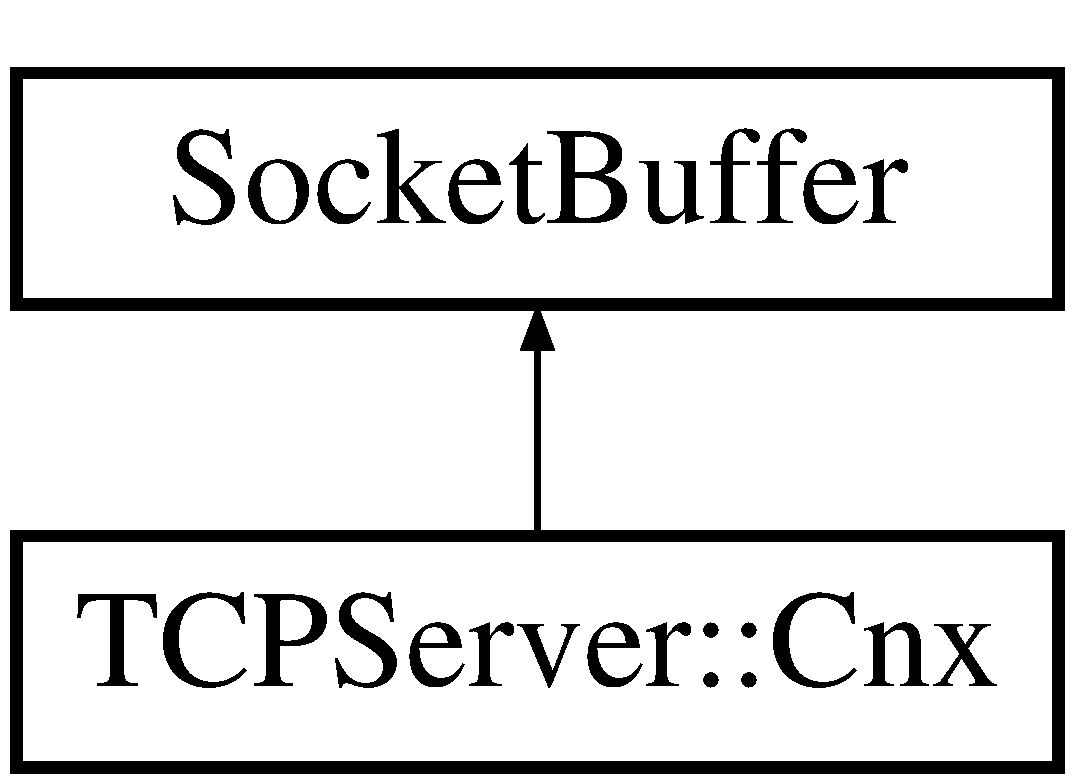
\includegraphics[height=2.000000cm]{classSocketBuffer}
\end{center}
\end{figure}
\subsection*{Public Member Functions}
\begin{DoxyCompactItemize}
\item 
\hypertarget{classSocketBuffer_aa9ed1cc8e166f53606b31246838b3d87}{\hyperlink{classSocketBuffer_aa9ed1cc8e166f53606b31246838b3d87}{Socket\-Buffer} (\hyperlink{classSocket}{Socket} $\ast$socket, size\-\_\-t input\-Buffer\-Size=8192, size\-\_\-t ouput\-Buffer\-Size=8192)}\label{classSocketBuffer_aa9ed1cc8e166f53606b31246838b3d87}

\begin{DoxyCompactList}\small\item\em constructor. The argument must be a valid connected T\-C\-P/\-I\-P \hyperlink{classSocket}{Socket} (i.\-e. of S\-O\-C\-K\-\_\-\-S\-T\-R\-E\-A\-M type) that must N\-O\-T be destructed while this \hyperlink{classSocketBuffer}{Socket\-Buffer} is used. \end{DoxyCompactList}\item 
\hypertarget{classSocketBuffer_a40ad003b90446f69fb0fa4cc18c0d28b}{{\bfseries Socket\-Buffer} (\hyperlink{classSocket}{Socket} \&socket, size\-\_\-t input\-Buffer\-Size=8192, size\-\_\-t ouput\-Buffer\-Size=8192)}\label{classSocketBuffer_a40ad003b90446f69fb0fa4cc18c0d28b}

\item 
\hypertarget{classSocketBuffer_aa9c14ec14e092fc58c4363d2bbc20ffd}{\hyperlink{classSocket}{Socket} $\ast$ {\bfseries socket} ()}\label{classSocketBuffer_aa9c14ec14e092fc58c4363d2bbc20ffd}

\item 
virtual void \hyperlink{classSocketBuffer_ac03353a864ab3a04aa25364a333c0a09}{set\-Separators} (int input\-Separator, int output\-Separator)
\begin{DoxyCompactList}\small\item\em changes the Line Separators. the argument is a character or a negative value (see below)\-: \end{DoxyCompactList}\item 
virtual void \hyperlink{classSocketBuffer_a81a280c639a913b5dbfb12611f339232}{get\-Separators} (int \&input\-Separator, int \&output\-Separator) const 
\begin{DoxyCompactList}\small\item\em returns the Line Separators. \end{DoxyCompactList}\item 
virtual ssize\-\_\-t \hyperlink{classSocketBuffer_a279a372ca946b58455dba0e9c12e213d}{read\-Line} (std\-::string \&str)
\begin{DoxyCompactList}\small\item\em Reads a line of text from a connected socket. The text is stored in the string given as an argument. The other side must send a line of text ended by a Line Separator (. \end{DoxyCompactList}\item 
virtual ssize\-\_\-t \hyperlink{classSocketBuffer_af589c1459da6bca39badf56798c6f859}{write\-Line} (const std\-::string \&str)
\begin{DoxyCompactList}\small\item\em Sends a line of text to a connected socket. Sends the string given as an argument. A Line Separator is automatically added (. \end{DoxyCompactList}\item 
\hypertarget{classSocketBuffer_ab77a4365cfb9625dc996005ffa22bc0c}{virtual ssize\-\_\-t {\bfseries read} (char $\ast$buffer, size\-\_\-t len)}\label{classSocketBuffer_ab77a4365cfb9625dc996005ffa22bc0c}

\item 
\hypertarget{classSocketBuffer_a2ceb624ffd27a27ef500574646c9a8fa}{virtual ssize\-\_\-t {\bfseries write} (const char $\ast$str, size\-\_\-t len)}\label{classSocketBuffer_a2ceb624ffd27a27ef500574646c9a8fa}

\end{DoxyCompactItemize}
\subsection*{Protected Member Functions}
\begin{DoxyCompactItemize}
\item 
\hypertarget{classSocketBuffer_ab2f6ba1d14564967e1714ddd478275d8}{virtual bool {\bfseries retrieve\-Line} (std\-::string \&str, ssize\-\_\-t received)}\label{classSocketBuffer_ab2f6ba1d14564967e1714ddd478275d8}

\end{DoxyCompactItemize}
\subsection*{Protected Attributes}
\begin{DoxyCompactItemize}
\item 
\hypertarget{classSocketBuffer_a19f587689e24a3900a4157be5fa27205}{size\-\_\-t {\bfseries \-\_\-in\-Size}}\label{classSocketBuffer_a19f587689e24a3900a4157be5fa27205}

\item 
\hypertarget{classSocketBuffer_a1ce4a460af7a7fb2f3609bcb9f15ece7}{size\-\_\-t {\bfseries \-\_\-out\-Size}}\label{classSocketBuffer_a1ce4a460af7a7fb2f3609bcb9f15ece7}

\item 
\hypertarget{classSocketBuffer_a8958b13b28d476081c10aac8e25a87d2}{int {\bfseries \-\_\-in\-Sep}}\label{classSocketBuffer_a8958b13b28d476081c10aac8e25a87d2}

\item 
\hypertarget{classSocketBuffer_add088335eb098a067980157b310b22cb}{int {\bfseries \-\_\-out\-Sep}}\label{classSocketBuffer_add088335eb098a067980157b310b22cb}

\item 
\hypertarget{classSocketBuffer_a8575c3a91db81fac18e5634c427faafb}{\hyperlink{classSocket}{Socket} $\ast$ {\bfseries \-\_\-sock}}\label{classSocketBuffer_a8575c3a91db81fac18e5634c427faafb}

\item 
\hypertarget{classSocketBuffer_a8cf67350de772512eff4af7d7f378bed}{struct \hyperlink{structInputBuffer}{Input\-Buffer} $\ast$ {\bfseries \-\_\-in}}\label{classSocketBuffer_a8cf67350de772512eff4af7d7f378bed}

\end{DoxyCompactItemize}


\subsection{Detailed Description}
Class for exchanging text strings between T\-C\-P/\-I\-P sockets. T\-C\-P/\-I\-P connected sockets do not preserve record boundaries. Messages can be split or merged so that one call to \hyperlink{classSocket_a9275eacdb64056a53cf4b9cf54cd2f1a}{Socket\-::send()} on the sending side does not necessarily correspond to one call to \hyperlink{classSocket_aa5e98b6f2c4e26fcf90d71c8386fc09d}{Socket\-::receive()} on the receiving side. 

The methods of this class solve this problem\-:
\begin{DoxyItemize}
\item by calling \hyperlink{classSocket_a9275eacdb64056a53cf4b9cf54cd2f1a}{Socket\-::send()} or \hyperlink{classSocket_aa5e98b6f2c4e26fcf90d71c8386fc09d}{Socket\-::receive()} as many times as needed
\item by using a Line Separator to separate text lines (\begin{DoxySeeAlso}{See Also}
set\-Separator()) 
\end{DoxySeeAlso}

\end{DoxyItemize}

\subsection{Member Function Documentation}
\hypertarget{classSocketBuffer_a81a280c639a913b5dbfb12611f339232}{\index{Socket\-Buffer@{Socket\-Buffer}!get\-Separators@{get\-Separators}}
\index{get\-Separators@{get\-Separators}!SocketBuffer@{Socket\-Buffer}}
\subsubsection[{get\-Separators}]{\setlength{\rightskip}{0pt plus 5cm}void Socket\-Buffer\-::get\-Separators (
\begin{DoxyParamCaption}
\item[{int \&}]{input\-Separator, }
\item[{int \&}]{output\-Separator}
\end{DoxyParamCaption}
) const\hspace{0.3cm}{\ttfamily [virtual]}}}\label{classSocketBuffer_a81a280c639a913b5dbfb12611f339232}


returns the Line Separators. 

\begin{DoxySeeAlso}{See Also}
\hyperlink{classSocketBuffer_ac03353a864ab3a04aa25364a333c0a09}{set\-Separators()}. 
\end{DoxySeeAlso}
\hypertarget{classSocketBuffer_a279a372ca946b58455dba0e9c12e213d}{\index{Socket\-Buffer@{Socket\-Buffer}!read\-Line@{read\-Line}}
\index{read\-Line@{read\-Line}!SocketBuffer@{Socket\-Buffer}}
\subsubsection[{read\-Line}]{\setlength{\rightskip}{0pt plus 5cm}ssize\-\_\-t Socket\-Buffer\-::read\-Line (
\begin{DoxyParamCaption}
\item[{std\-::string \&}]{str}
\end{DoxyParamCaption}
)\hspace{0.3cm}{\ttfamily [virtual]}}}\label{classSocketBuffer_a279a372ca946b58455dba0e9c12e213d}


Reads a line of text from a connected socket. The text is stored in the string given as an argument. The other side must send a line of text ended by a Line Separator (. 

\begin{DoxySeeAlso}{See Also}
set\-Separator()) which is automatically done by \hyperlink{classSocketBuffer_af589c1459da6bca39badf56798c6f859}{write\-Line()}. The separator is not stored in the argument. 
\end{DoxySeeAlso}
\begin{DoxyReturn}{Returns}
the number of bytes that was received (including the separator) except if\-:
\begin{DoxyItemize}
\item shutdown\-Output() was called on the other side (0 is returned)
\item an error occured (Socket\-::\-Failed is returned)
\item the socket is invalid (Socket\-::\-Invalid\-Socket is returned) 
\end{DoxyItemize}
\end{DoxyReturn}
\begin{DoxyNote}{Note}
this method may block. 
\end{DoxyNote}
\hypertarget{classSocketBuffer_ac03353a864ab3a04aa25364a333c0a09}{\index{Socket\-Buffer@{Socket\-Buffer}!set\-Separators@{set\-Separators}}
\index{set\-Separators@{set\-Separators}!SocketBuffer@{Socket\-Buffer}}
\subsubsection[{set\-Separators}]{\setlength{\rightskip}{0pt plus 5cm}void Socket\-Buffer\-::set\-Separators (
\begin{DoxyParamCaption}
\item[{int}]{input\-Separator, }
\item[{int}]{output\-Separator}
\end{DoxyParamCaption}
)\hspace{0.3cm}{\ttfamily [virtual]}}}\label{classSocketBuffer_ac03353a864ab3a04aa25364a333c0a09}


changes the Line Separators. the argument is a character or a negative value (see below)\-: 


\begin{DoxyItemize}
\item if {\itshape input\-Separator} is $<$ 0 (the default) a line is considered to be terminated by any one of '\par
' or '' or '\par
' followed by ''
\item if {\itshape output\-Separator} is $<$ 0 a line is terminated by '\par
' followed by ''. The default value is '\par
'. 
\end{DoxyItemize}\hypertarget{classSocketBuffer_af589c1459da6bca39badf56798c6f859}{\index{Socket\-Buffer@{Socket\-Buffer}!write\-Line@{write\-Line}}
\index{write\-Line@{write\-Line}!SocketBuffer@{Socket\-Buffer}}
\subsubsection[{write\-Line}]{\setlength{\rightskip}{0pt plus 5cm}ssize\-\_\-t Socket\-Buffer\-::write\-Line (
\begin{DoxyParamCaption}
\item[{const std\-::string \&}]{str}
\end{DoxyParamCaption}
)\hspace{0.3cm}{\ttfamily [virtual]}}}\label{classSocketBuffer_af589c1459da6bca39badf56798c6f859}


Sends a line of text to a connected socket. Sends the string given as an argument. A Line Separator is automatically added (. 

\begin{DoxySeeAlso}{See Also}
set\-Separator()). 
\end{DoxySeeAlso}
\begin{DoxyReturn}{Returns}
the number of bytes that was sent (including the separator) except if\-:
\begin{DoxyItemize}
\item shutdown\-Input() was called on the other side (0 is returned)
\item an error occured (Socket\-::\-Failed is returned)
\item the socket is invalid (Socket\-::\-Invalid\-Socket is returned) 
\end{DoxyItemize}
\end{DoxyReturn}
\begin{DoxyNote}{Note}
this method may block. 
\end{DoxyNote}


The documentation for this class was generated from the following files\-:\begin{DoxyCompactItemize}
\item 
Socket.\-h\item 
Socket.\-cpp\end{DoxyCompactItemize}

\hypertarget{classTCPServer}{\section{T\-C\-P\-Server Class Reference}
\label{classTCPServer}\index{T\-C\-P\-Server@{T\-C\-P\-Server}}
}


T\-C\-P/\-I\-P I\-Pv4 server. The server supports T\-C\-P/\-I\-P A\-F\-\_\-\-I\-N\-E\-T connections (following the I\-Pv4 Internet protocol) with multiple clients. One thread is used per client.  




{\ttfamily \#include $<$T\-C\-P\-Server.\-h$>$}

\subsection*{Classes}
\begin{DoxyCompactItemize}
\item 
class \hyperlink{classTCPServer_1_1Callback}{Callback}
\item 
class \hyperlink{classTCPServer_1_1CallbackImpl}{Callback\-Impl}
\item 
class \hyperlink{classTCPServer_1_1Cnx}{Cnx}
\begin{DoxyCompactList}\small\item\em represents a connection with a given client. \end{DoxyCompactList}\item 
class \hyperlink{classTCPServer_1_1Lock}{Lock}
\begin{DoxyCompactList}\small\item\em locks the server in read mode or in write mode. In order to avoid concurrency problems between threads, the callback method that processes requests should instantiate a \hyperlink{classTCPServer_1_1Lock}{Lock} object in the stack. The \hyperlink{classTCPServer_1_1Lock}{Lock} must be instantiated in write mode if the request changes data, or in read mode otherwise. A write lock blocks all other locks (hence, all other threads) until the callback method that issued the write lock returns. \end{DoxyCompactList}\end{DoxyCompactItemize}
\subsection*{Public Member Functions}
\begin{DoxyCompactItemize}
\item 
\hypertarget{classTCPServer_a3a5e3cfe42c676ed71f2bc58dcc92bda}{\hyperlink{classTCPServer_a3a5e3cfe42c676ed71f2bc58dcc92bda}{T\-C\-P\-Server} ()}\label{classTCPServer_a3a5e3cfe42c676ed71f2bc58dcc92bda}

\begin{DoxyCompactList}\small\item\em constructor\-: initializes the \hyperlink{classTCPServer}{T\-C\-P\-Server}. \end{DoxyCompactList}\item 
\hypertarget{classTCPServer_abc497ac52355e53986a6a1bd1acb9581}{virtual \hyperlink{classTCPServer_abc497ac52355e53986a6a1bd1acb9581}{$\sim$\-T\-C\-P\-Server} ()}\label{classTCPServer_abc497ac52355e53986a6a1bd1acb9581}

\begin{DoxyCompactList}\small\item\em destructor\-: cleans up the \hyperlink{classTCPServer}{T\-C\-P\-Server}. \end{DoxyCompactList}\item 
virtual int \hyperlink{classTCPServer_a1409041961e91f1dbc4933483b4c3b23}{run} (int port)
\begin{DoxyCompactList}\small\item\em starts the main loop of the server on this port. This function binds an internal \hyperlink{classServerSocket}{Server\-Socket} then starts an infinite main loop that receives requests from clients. The function creates one thread per client. \end{DoxyCompactList}\item 
{\footnotesize template$<$class T $>$ }\\void \hyperlink{classTCPServer_ac62c8c7a1d1137b74e2a1fa6d8a4a876}{set\-Callback} (T $\ast$obj, bool(T\-::$\ast$func)(\hyperlink{classTCPServer_1_1Cnx}{Cnx} \&, const std\-::string \&request, std\-::string \&response))
\begin{DoxyCompactList}\small\item\em changes the callback method that processes requests. The first argument must be an object, the second argument a method of this object. This method will be called each time the \hyperlink{classTCPServer}{T\-C\-P\-Server} receives a 'request' from a client in order to perform a computation and return a 'response' to this client. \end{DoxyCompactList}\end{DoxyCompactItemize}
\subsection*{Protected Member Functions}
\begin{DoxyCompactItemize}
\item 
\hypertarget{classTCPServer_af99977f3ec05210e91d02aa9c693254b}{virtual void \hyperlink{classTCPServer_af99977f3ec05210e91d02aa9c693254b}{read\-Messages} (\hyperlink{classTCPServer_1_1Cnx}{T\-C\-P\-Server\-::\-Cnx} $\ast$)}\label{classTCPServer_af99977f3ec05210e91d02aa9c693254b}

\begin{DoxyCompactList}\small\item\em reads messages from a given client on the corresponding thread. \end{DoxyCompactList}\item 
\hypertarget{classTCPServer_a2f053dfc720aab308f97ccc8a789adc4}{virtual void \hyperlink{classTCPServer_a2f053dfc720aab308f97ccc8a789adc4}{print\-Msg} (const std\-::string \&msg, const \hyperlink{classTCPServer_1_1Cnx}{T\-C\-P\-Server\-::\-Cnx} $\ast$=0)}\label{classTCPServer_a2f053dfc720aab308f97ccc8a789adc4}

\begin{DoxyCompactList}\small\item\em prints warning and error messages on the terminal. \end{DoxyCompactList}\end{DoxyCompactItemize}
\subsection*{Protected Attributes}
\begin{DoxyCompactItemize}
\item 
\hypertarget{classTCPServer_a9c2891cf40b19735bceb22605a5e867e}{\hyperlink{classServerSocket}{Server\-Socket} {\bfseries \-\_\-servsock}}\label{classTCPServer_a9c2891cf40b19735bceb22605a5e867e}

\item 
\hypertarget{classTCPServer_a1f7a87b1f42950325d005c8a0ca9427e}{std\-::shared\-\_\-ptr$<$ \hyperlink{classTCPServer_1_1Callback}{Callback} $>$ {\bfseries \-\_\-callback}}\label{classTCPServer_a1f7a87b1f42950325d005c8a0ca9427e}

\item 
\hypertarget{classTCPServer_a130152438b313a1c4470c842a063257d}{pthread\-\_\-rwlock\-\_\-t {\bfseries \-\_\-threadlock}}\label{classTCPServer_a130152438b313a1c4470c842a063257d}

\end{DoxyCompactItemize}


\subsection{Detailed Description}
T\-C\-P/\-I\-P I\-Pv4 server. The server supports T\-C\-P/\-I\-P A\-F\-\_\-\-I\-N\-E\-T connections (following the I\-Pv4 Internet protocol) with multiple clients. One thread is used per client. 

The \hyperlink{classTCPServer_a1409041961e91f1dbc4933483b4c3b23}{run()} method binds an internal \hyperlink{classServerSocket}{Server\-Socket} then starts an infinite main loop that receives requests from clients. Requests can be received concurrently thanks to threads.

A callback method is called each time the sever receives a request from a client (\begin{DoxySeeAlso}{See Also}
\hyperlink{classTCPServer_ac62c8c7a1d1137b74e2a1fa6d8a4a876}{set\-Callback()} to set this method). This method can issue read and write locks to avoid concurrency issues (

\hyperlink{classTCPServer_1_1Lock}{Lock}). 
\end{DoxySeeAlso}


\subsection{Member Function Documentation}
\hypertarget{classTCPServer_a1409041961e91f1dbc4933483b4c3b23}{\index{T\-C\-P\-Server@{T\-C\-P\-Server}!run@{run}}
\index{run@{run}!TCPServer@{T\-C\-P\-Server}}
\subsubsection[{run}]{\setlength{\rightskip}{0pt plus 5cm}int T\-C\-P\-Server\-::run (
\begin{DoxyParamCaption}
\item[{int}]{port}
\end{DoxyParamCaption}
)\hspace{0.3cm}{\ttfamily [virtual]}}}\label{classTCPServer_a1409041961e91f1dbc4933483b4c3b23}


starts the main loop of the server on this port. This function binds an internal \hyperlink{classServerSocket}{Server\-Socket} then starts an infinite main loop that receives requests from clients. The function creates one thread per client. 

\begin{DoxyReturn}{Returns}
0 on normal termination or a negative value if the \hyperlink{classServerSocket}{Server\-Socket} could not be bound (value is then one of \hyperlink{classSocket_a9f68308228badcdd299cd83e62e36976}{Socket\-::\-Errors}). 
\end{DoxyReturn}
\hypertarget{classTCPServer_ac62c8c7a1d1137b74e2a1fa6d8a4a876}{\index{T\-C\-P\-Server@{T\-C\-P\-Server}!set\-Callback@{set\-Callback}}
\index{set\-Callback@{set\-Callback}!TCPServer@{T\-C\-P\-Server}}
\subsubsection[{set\-Callback}]{\setlength{\rightskip}{0pt plus 5cm}template$<$class T $>$ void T\-C\-P\-Server\-::set\-Callback (
\begin{DoxyParamCaption}
\item[{T $\ast$}]{obj, }
\item[{bool(T\-::$\ast$)({\bf Cnx} \&, const std\-::string \&request, std\-::string \&response)}]{func}
\end{DoxyParamCaption}
)\hspace{0.3cm}{\ttfamily [inline]}}}\label{classTCPServer_ac62c8c7a1d1137b74e2a1fa6d8a4a876}


changes the callback method that processes requests. The first argument must be an object, the second argument a method of this object. This method will be called each time the \hyperlink{classTCPServer}{T\-C\-P\-Server} receives a 'request' from a client in order to perform a computation and return a 'response' to this client. 

Arguments and return value of the method\-:
\begin{DoxyItemize}
\item the 'request' and the 'response' are provided through the corresponding parameters of the method.
\item the connection with the client will be closed if the method returns false 
\end{DoxyItemize}

The documentation for this class was generated from the following files\-:\begin{DoxyCompactItemize}
\item 
T\-C\-P\-Server.\-h\item 
T\-C\-P\-Server.\-cpp\end{DoxyCompactItemize}

\hypertarget{classVideo}{\section{Video Class Reference}
\label{classVideo}\index{Video@{Video}}
}


The \hyperlink{classVideo}{Video} class params\-: duree\-: int methods\-: \hyperlink{classVideo_af9bf19109d8c613426173524942a59f0}{set\-Duree(int d)} \hyperlink{classVideo_a6ce28ec6b467212e7bb3cbf635b57598}{get\-Duree()} \hyperlink{classVideo_af6a8d2f22330651f3f264292e580dca3}{open\-Object()} \hyperlink{classVideo_a180c985ff368f77d0fb66ec106106f00}{affichage(ostream \&s)}  




{\ttfamily \#include $<$video.\-h$>$}

Inheritance diagram for Video\-:\begin{figure}[H]
\begin{center}
\leavevmode
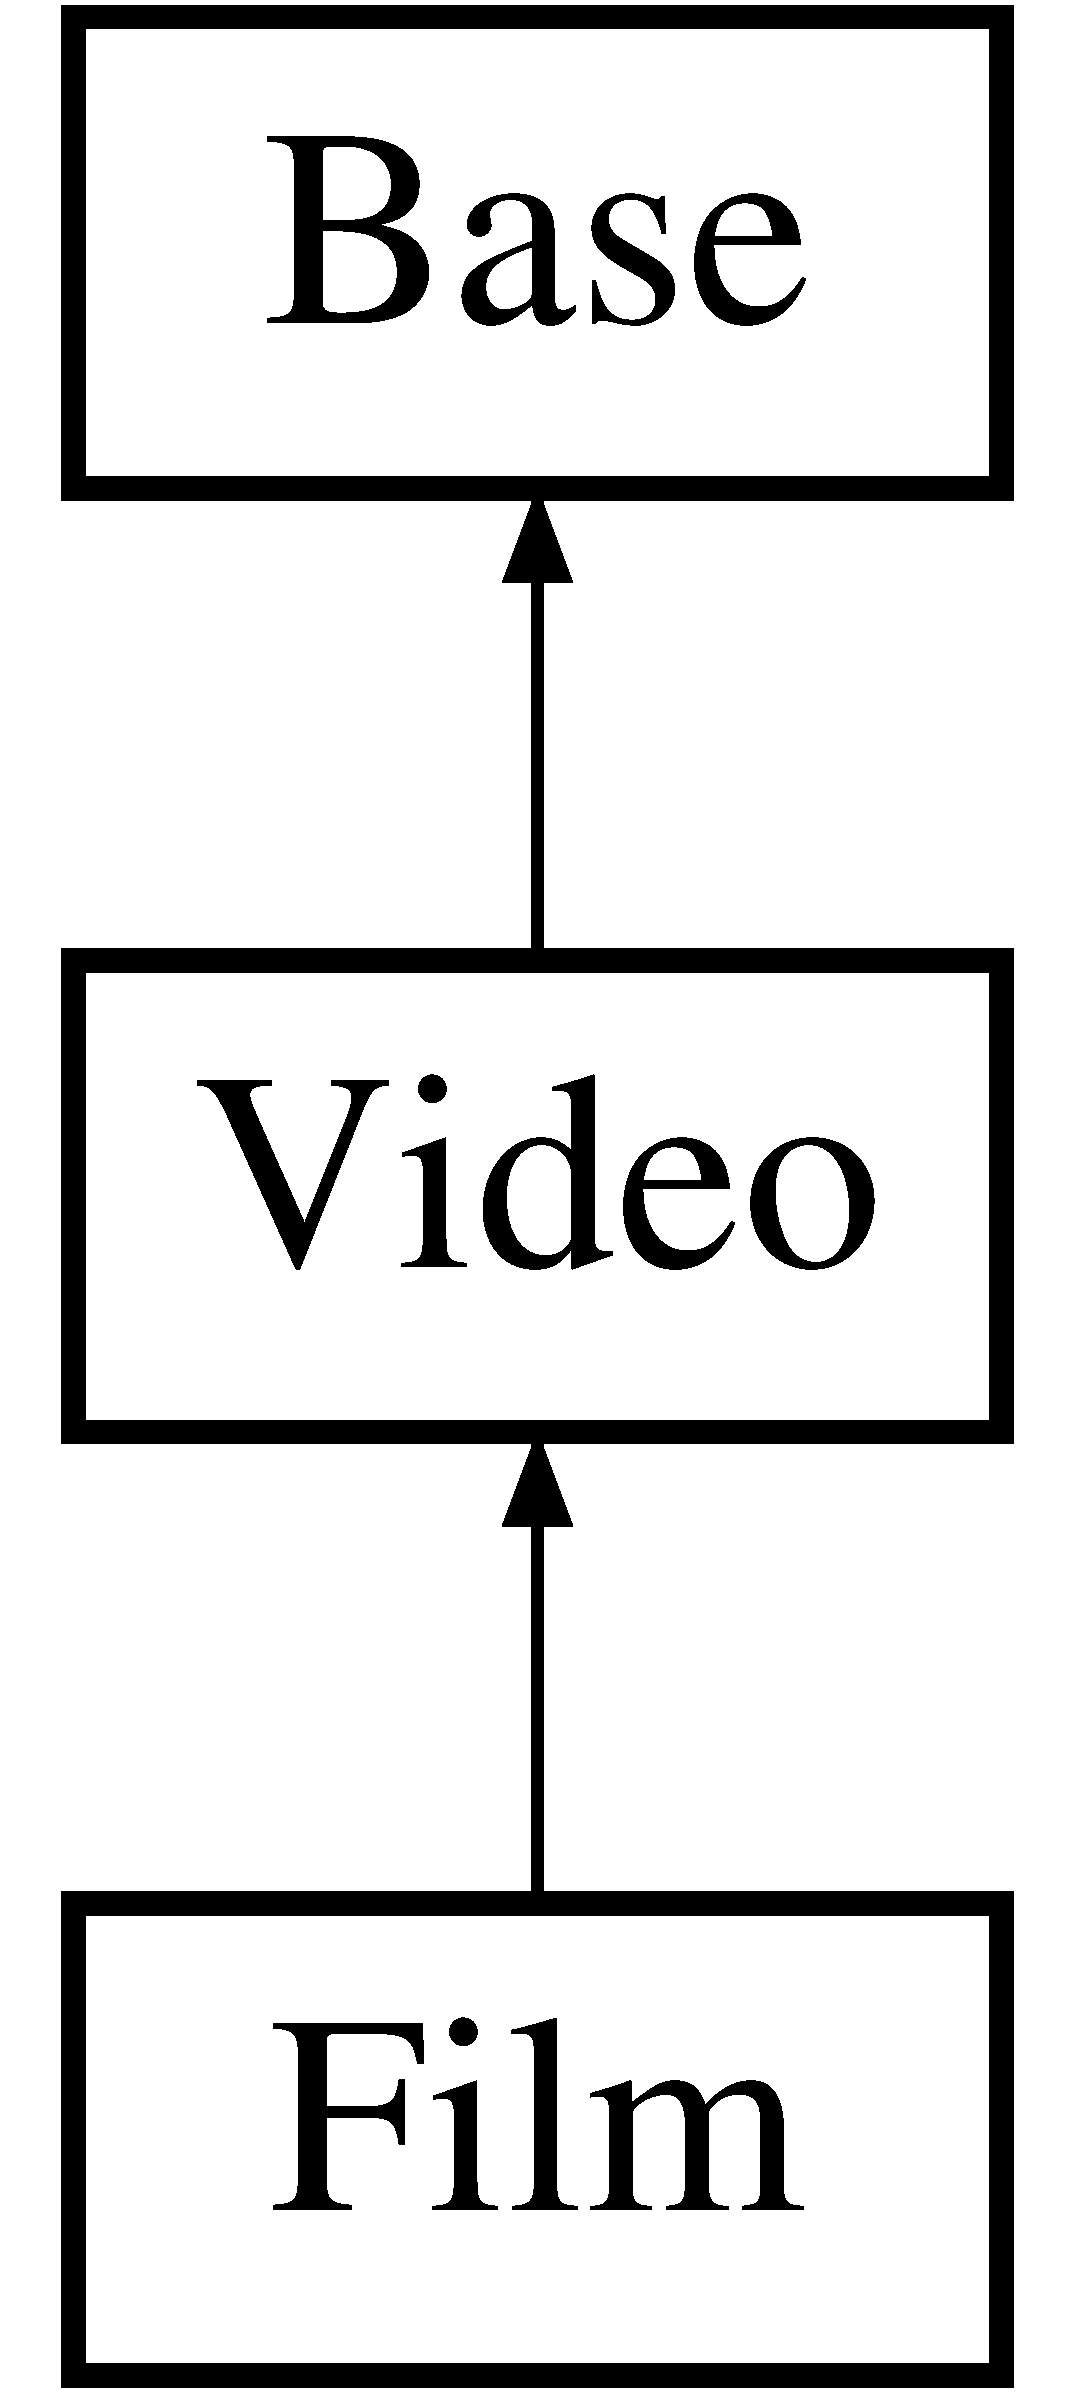
\includegraphics[height=3.000000cm]{classVideo}
\end{center}
\end{figure}
\subsection*{Public Member Functions}
\begin{DoxyCompactItemize}
\item 
\hypertarget{classVideo_ab67336c2c5b6227a9635bc7dcd6af543}{\hyperlink{classVideo_ab67336c2c5b6227a9635bc7dcd6af543}{Video} ()}\label{classVideo_ab67336c2c5b6227a9635bc7dcd6af543}

\begin{DoxyCompactList}\small\item\em \hyperlink{classVideo}{Video} Constructor overcharge. \end{DoxyCompactList}\item 
\hyperlink{classVideo_ab5a0624db51e978d6d87aa40012885d7}{Video} (string name, string pathname, int duree)
\begin{DoxyCompactList}\small\item\em \hyperlink{classVideo}{Video} Constructor. \end{DoxyCompactList}\item 
virtual void \hyperlink{classVideo_af9bf19109d8c613426173524942a59f0}{set\-Duree} (int d)
\begin{DoxyCompactList}\small\item\em set\-Duree \end{DoxyCompactList}\item 
virtual int \hyperlink{classVideo_a6ce28ec6b467212e7bb3cbf635b57598}{get\-Duree} () const 
\begin{DoxyCompactList}\small\item\em get\-Duree \end{DoxyCompactList}\item 
\hypertarget{classVideo_af6a8d2f22330651f3f264292e580dca3}{virtual void \hyperlink{classVideo_af6a8d2f22330651f3f264292e580dca3}{open\-Object} ()}\label{classVideo_af6a8d2f22330651f3f264292e580dca3}

\begin{DoxyCompactList}\small\item\em open\-Object Plays video using xdg-\/open (opens with default program). As with \hyperlink{classPhoto}{Photo}, there was a problem using the \& and did not weork properly, with this solution it seems to be solved \end{DoxyCompactList}\item 
virtual string \hyperlink{classVideo_a180c985ff368f77d0fb66ec106106f00}{affichage} (ostream \&s) override
\begin{DoxyCompactList}\small\item\em affichage \end{DoxyCompactList}\item 
\hypertarget{classVideo_a07a39b94dddfa02e0b0d7b196e9c9f53}{virtual \hyperlink{classVideo_a07a39b94dddfa02e0b0d7b196e9c9f53}{$\sim$\-Video} ()}\label{classVideo_a07a39b94dddfa02e0b0d7b196e9c9f53}

\begin{DoxyCompactList}\small\item\em $\sim$\-Video Destructor \end{DoxyCompactList}\end{DoxyCompactItemize}


\subsection{Detailed Description}
The \hyperlink{classVideo}{Video} class params\-: duree\-: int methods\-: \hyperlink{classVideo_af9bf19109d8c613426173524942a59f0}{set\-Duree(int d)} \hyperlink{classVideo_a6ce28ec6b467212e7bb3cbf635b57598}{get\-Duree()} \hyperlink{classVideo_af6a8d2f22330651f3f264292e580dca3}{open\-Object()} \hyperlink{classVideo_a180c985ff368f77d0fb66ec106106f00}{affichage(ostream \&s)} 

\subsection{Constructor \& Destructor Documentation}
\hypertarget{classVideo_ab5a0624db51e978d6d87aa40012885d7}{\index{Video@{Video}!Video@{Video}}
\index{Video@{Video}!Video@{Video}}
\subsubsection[{Video}]{\setlength{\rightskip}{0pt plus 5cm}Video\-::\-Video (
\begin{DoxyParamCaption}
\item[{string}]{name, }
\item[{string}]{pathname, }
\item[{int}]{duree}
\end{DoxyParamCaption}
)\hspace{0.3cm}{\ttfamily [inline]}}}\label{classVideo_ab5a0624db51e978d6d87aa40012885d7}


\hyperlink{classVideo}{Video} Constructor. 


\begin{DoxyParams}{Parameters}
{\em name} & string \\
\hline
{\em pathname} & string \\
\hline
{\em duree} & int \\
\hline
\end{DoxyParams}


\subsection{Member Function Documentation}
\hypertarget{classVideo_a180c985ff368f77d0fb66ec106106f00}{\index{Video@{Video}!affichage@{affichage}}
\index{affichage@{affichage}!Video@{Video}}
\subsubsection[{affichage}]{\setlength{\rightskip}{0pt plus 5cm}virtual string Video\-::affichage (
\begin{DoxyParamCaption}
\item[{ostream \&}]{s}
\end{DoxyParamCaption}
)\hspace{0.3cm}{\ttfamily [inline]}, {\ttfamily [override]}, {\ttfamily [virtual]}}}\label{classVideo_a180c985ff368f77d0fb66ec106106f00}


affichage 


\begin{DoxyParams}{Parameters}
{\em s} & ostream \\
\hline
\end{DoxyParams}
\begin{DoxyReturn}{Returns}
string of attributes of video Prints through s the returned string 
\end{DoxyReturn}


Reimplemented from \hyperlink{classBase_ad712ff856464b0d3fa96d07eae70a90e}{Base}.



Reimplemented in \hyperlink{classFilm_a0fd2b4ba12627d9268fb0ee64b850b15}{Film}.

\hypertarget{classVideo_a6ce28ec6b467212e7bb3cbf635b57598}{\index{Video@{Video}!get\-Duree@{get\-Duree}}
\index{get\-Duree@{get\-Duree}!Video@{Video}}
\subsubsection[{get\-Duree}]{\setlength{\rightskip}{0pt plus 5cm}virtual int Video\-::get\-Duree (
\begin{DoxyParamCaption}
{}
\end{DoxyParamCaption}
) const\hspace{0.3cm}{\ttfamily [inline]}, {\ttfamily [virtual]}}}\label{classVideo_a6ce28ec6b467212e7bb3cbf635b57598}


get\-Duree 

\begin{DoxyReturn}{Returns}
duree int (duration of video) 
\end{DoxyReturn}
\hypertarget{classVideo_af9bf19109d8c613426173524942a59f0}{\index{Video@{Video}!set\-Duree@{set\-Duree}}
\index{set\-Duree@{set\-Duree}!Video@{Video}}
\subsubsection[{set\-Duree}]{\setlength{\rightskip}{0pt plus 5cm}virtual void Video\-::set\-Duree (
\begin{DoxyParamCaption}
\item[{int}]{d}
\end{DoxyParamCaption}
)\hspace{0.3cm}{\ttfamily [inline]}, {\ttfamily [virtual]}}}\label{classVideo_af9bf19109d8c613426173524942a59f0}


set\-Duree 


\begin{DoxyParams}{Parameters}
{\em d} & int Sets duree to the value of d \\
\hline
\end{DoxyParams}


The documentation for this class was generated from the following file\-:\begin{DoxyCompactItemize}
\item 
video.\-h\end{DoxyCompactItemize}

%--- End generated contents ---

% Index
\newpage
\phantomsection
\addcontentsline{toc}{chapter}{Index}
\printindex

\end{document}
